\documentclass[pdftex,cyrillic,14pt,a4page,twoside,openright]{extreport}
\usepackage[bulgarian]{babel}

\usepackage[margin=2cm]{geometry}% http://ctan.org/pkg/geometry
\usepackage[pdftex]{graphicx}
\usepackage{hyperref}
\graphicspath{ {./figures/} }

\usepackage{./titlesec/titlesec}

% Counter too wide line spacing added by twoside
% https://tex.stackexchange.com/questions/62572/twoside-introduces-incorrect-linespacing-at-end-of-section
\raggedbottom
  
\titleformat{\chapter}%
  {\normalfont\bfseries\Huge}{\thechapter.}{10pt}{}

\usepackage{afterpage}
\newcommand\blankpage{%
    \null
    \thispagestyle{empty}%
    \newpage}


\begin{document}
\begin{titlepage}
	\begin{center}
	
\includegraphics[scale=1.2]{./NBU_logo.jpg}\\[0.3cm]
    \textbf{\Large НОВ БЪЛГАРСКИ УНИВЕРСИТЕТ\\[0.4cm]}
    \textbf{\Large Департамент Информатика\\[0.4cm]}
    \textbf{\Large Бакалавърка програма Информатика\\[3cm]}
   
		\textbf{\LARGE Автоматизиран биоинформатичен анализ на генетични варианти, потенциално свързани със стареенето\\[2cm]}
		\begin{Large}
		Дипломна работа на\\[0.2cm]
		Михаил М. Здравков\\[3cm]
		\end{Large}
		\begin{minipage}{0.48\textwidth}
			\begin{flushleft} \large
				\emph{Научни ръководители:} \\
				доц. д-р Милена Георгиева \\
				Момчил Топалов
			\end{flushleft}
		\end{minipage}
			\begin{minipage}{0.48\textwidth}
			\begin{flushright} \large
				\emph{Дипломен консултант:} \\
				гл. ас. д-р Методи Трайков\\
				\clearpage
			\end{flushright}
		\end{minipage}

		\vfill

		% Bottom of the page
		{\large София 2022}

	\end{center}
\end{titlepage}


\afterpage{\blankpage}

\newgeometry{
	inner=30mm,
    outer=20mm,
    top=20mm,
    bottom=20mm}

\tableofcontents
\pagebreak
%\afterpage{\blankpage}

\setlength\parindent{0pt}

\chapter*{Използвани съкращения}
\textbf{HGVS} - Human Genome Variation Society. Организация, занимаваща се с генетични варианти при хората, дала името и на стандартна номенклатура за описване на варианти на ДНК, РНК, протеини и други свързани с генетиката макромолекули.\\
\textbf{Indel} - Isertion/Deletion. Генни варианти, при които определена нуклеотидна последователност е изтрита или вмъкната.\\
\textbf{MNP} - Multiple Nucleotide Polymorphism. Множествен нуклеотиден полиморфизъм се нарича когато варианта и референтната поредица имат еднаква дължина, различна от 1.\\
\textbf{NGS} -  Next-Generation Sequencing - Технологии за секвениране от ново поколение.\\
\textbf{OLAP} - Online Analytical Processing. Aнализът в реално време е подход за бързо обработване на многомерни аналитични заявки.\\
\textbf{SNP} - Single Nucleotide Polymorphism. Единичен нуклеотиден полиморфизъм е тип мутация, наричана още точкова мутация, при която една единствена нуклеотидна база е променена.\\
\textbf{VCF} - Variant Call Format. Стандартен файлов формат за описване на генни варианти спрямо определен референтен геном.\\

\chapter{Увод}
\paragraph{}

Стареенето е естествен процес, който има огромно значение както за отделния индивид, така и за обществото като цяло. С напредването на възрастта, рискът от разнообразни заболявания като рак, болест на Алцхаймер, диабет, сърдечно-съдови заболявания и други нараства значително. Смята се, че около две-трети от смъртните случаи при хора се дължат на заболявания, свързани с възрастта. Същевременно, с глобалното нарастване на средната продължителност на живота, проблемите на стареенето засягат все повече хора и имат все по-голямо обществено значение. От социална гледна точка, стареенето оказва значителен икономически и демографски ефект. Тези проблеми превръщат търсенето на терапии за забавянето на стареенето и за справяне с негативните му ефекти в една от най-важните сфери на изследване в съвременната биология.

\paragraph{}
Въпреки все по-големите средства и усилия, които се влагат в изследване на стареенето, процесът все още остава недостатъчно добре разбран. Това се дължи на голямата сложност на този биологичен процес и на изобилието от механизми, които участват в него. Установено е, че той се влияе от множество генетични и епигенетични фактори.
Настоящата дипломна работа се фокусира върху генетичната основа на стареенето. В тази област се търсят кои са гените, които контролират стареенето, как правят това и съществуват ли техни варианти, които водят до подобряване или влошаване на фенотипа. Важен метод за изследването на тези въпроси е анализът на генетични варианти. За целта, секвениран геном се сравнява с определен референтен такъв, за да се намери как те се различават. Това създава голямо количество данни, които трябва да бъдат анализирани. Налични са множество различни биоинформатични инструменти, покриващи различни аспекти от обработката на файлове с генетични варианти - анотация, филтриране, анализ и т.н. Повечето от тях, обаче, изискват значителни технически познания, което ги прави трудни за използване от специалисти в други области, като биология и генетика.

\paragraph{}
Целта на настоящата дипломна работа е да се проектира и създаде интегрирана софтуерна система, която позволява на потребители без задълбочени познания по информатика да провеждат изследвания на генетични варианти по лесен и удобен начин.
            
\chapter{Литературен обзор}
\section{Значение на стареенето}
\subsection{Дефиниция}
\paragraph{}
Въпреки, че концепцията за стареене е универсално разбираема, формалната ѝ дефиниция не е тривиална и множество автори дават твърде различни определения за този термин. Аркинг (2006, стр. 11) прави преглед на наличната литература и, в резултат, предлага следната дефиниция \cite{arking2006biology}:

\paragraph{}
\textit{„Стареенето е независима от времето поредица от кумулативни, прогресивни, свойствени и вредящи структурни и функционални промени, които обикновено започват да се изразяват при репродуктивната зрялост и приключват със смъртта.“}

\paragraph{}
Макар времето да няма каузална връзка с ефектите на стареенето, то корелацията помежду им е причина обикновено да се говори за ефектите на стареенето като за нещо, настъпващо с напредването на възрастта.

\subsection{Физиологични ефекти}
\paragraph{}
Стареенето оказва изключително голям ефект върху човешкото тяло. То обикновено включва широк спектър от различни физиологични промени, които влошават жизнеността и качеството на живот на индивида. Примери за това са понижена фертилност при жените \cite{kamath2010}; загуба на телесна маса \cite{spencer1996}; влошен слух\cite{feder2015}; повишен риск от хронични заболявания \cite{larson2013}\cite{prasad2012}; хронична болка \cite{geriatrics2002}; загуба на сила и еластичност в мускулно-скелетната система; понижената способност за устояване на инфекции, екстремни температури и др. видове стрес; влошаване на зрението; загуба на неврологични функции \cite{vina2007} и други.

\paragraph{}
Тези физиологични промени водят до увеличен риск от редица заболявания, които съответно са най-често срещани сред възрастни хора. Една от основните промени, които настъпват по време на стареенето, е нарушената регулация на имунния отговор, което води до хронично системно възпалително състояние \cite{curwen2004}. Много проучвания показват, че хроничното възпаление може да има сериозна роля в широк спектър от свързани с възрастта заболявания, включително рак, диабет, сърдечносъдови, белодробни, невологични и автоимунни заболявания \cite{khansari2009}\cite{kuzhuvelil2008}.

\subsection{Демографски и икономически ефекти}
\paragraph{}
През последния един век очакваната продължителност на живота в целия свят драстично се е повишила \cite{zijdeman2016} (виж фиг. \ref{fig:life_expectancy}). Освен безспорните ползи, това води и до редица проблеми. Удължаването на продължителността на живота, в комбинация с наблюдавания спад на раждаемостта, се очаква да доведе до застаряване на населението \cite{lutz2008}. Световната Здравна Организация (СЗО) предупреждава, че се очаква между 2015 и 2050 броят на хората над 60-годишна възраст да се повиши от 12\% от населението до 22\% \cite{who_report_ageing2015}. Същевременно, по данни на СЗО, увеличаването на продължителността на живота (с 6 години за периода между 2000 и 2019) изпреварва увеличаването в продължителността на здравословния живот (с 5.4 години за същия период) \cite{who_health2020}.

\begin{figure}[h]
  \centering
  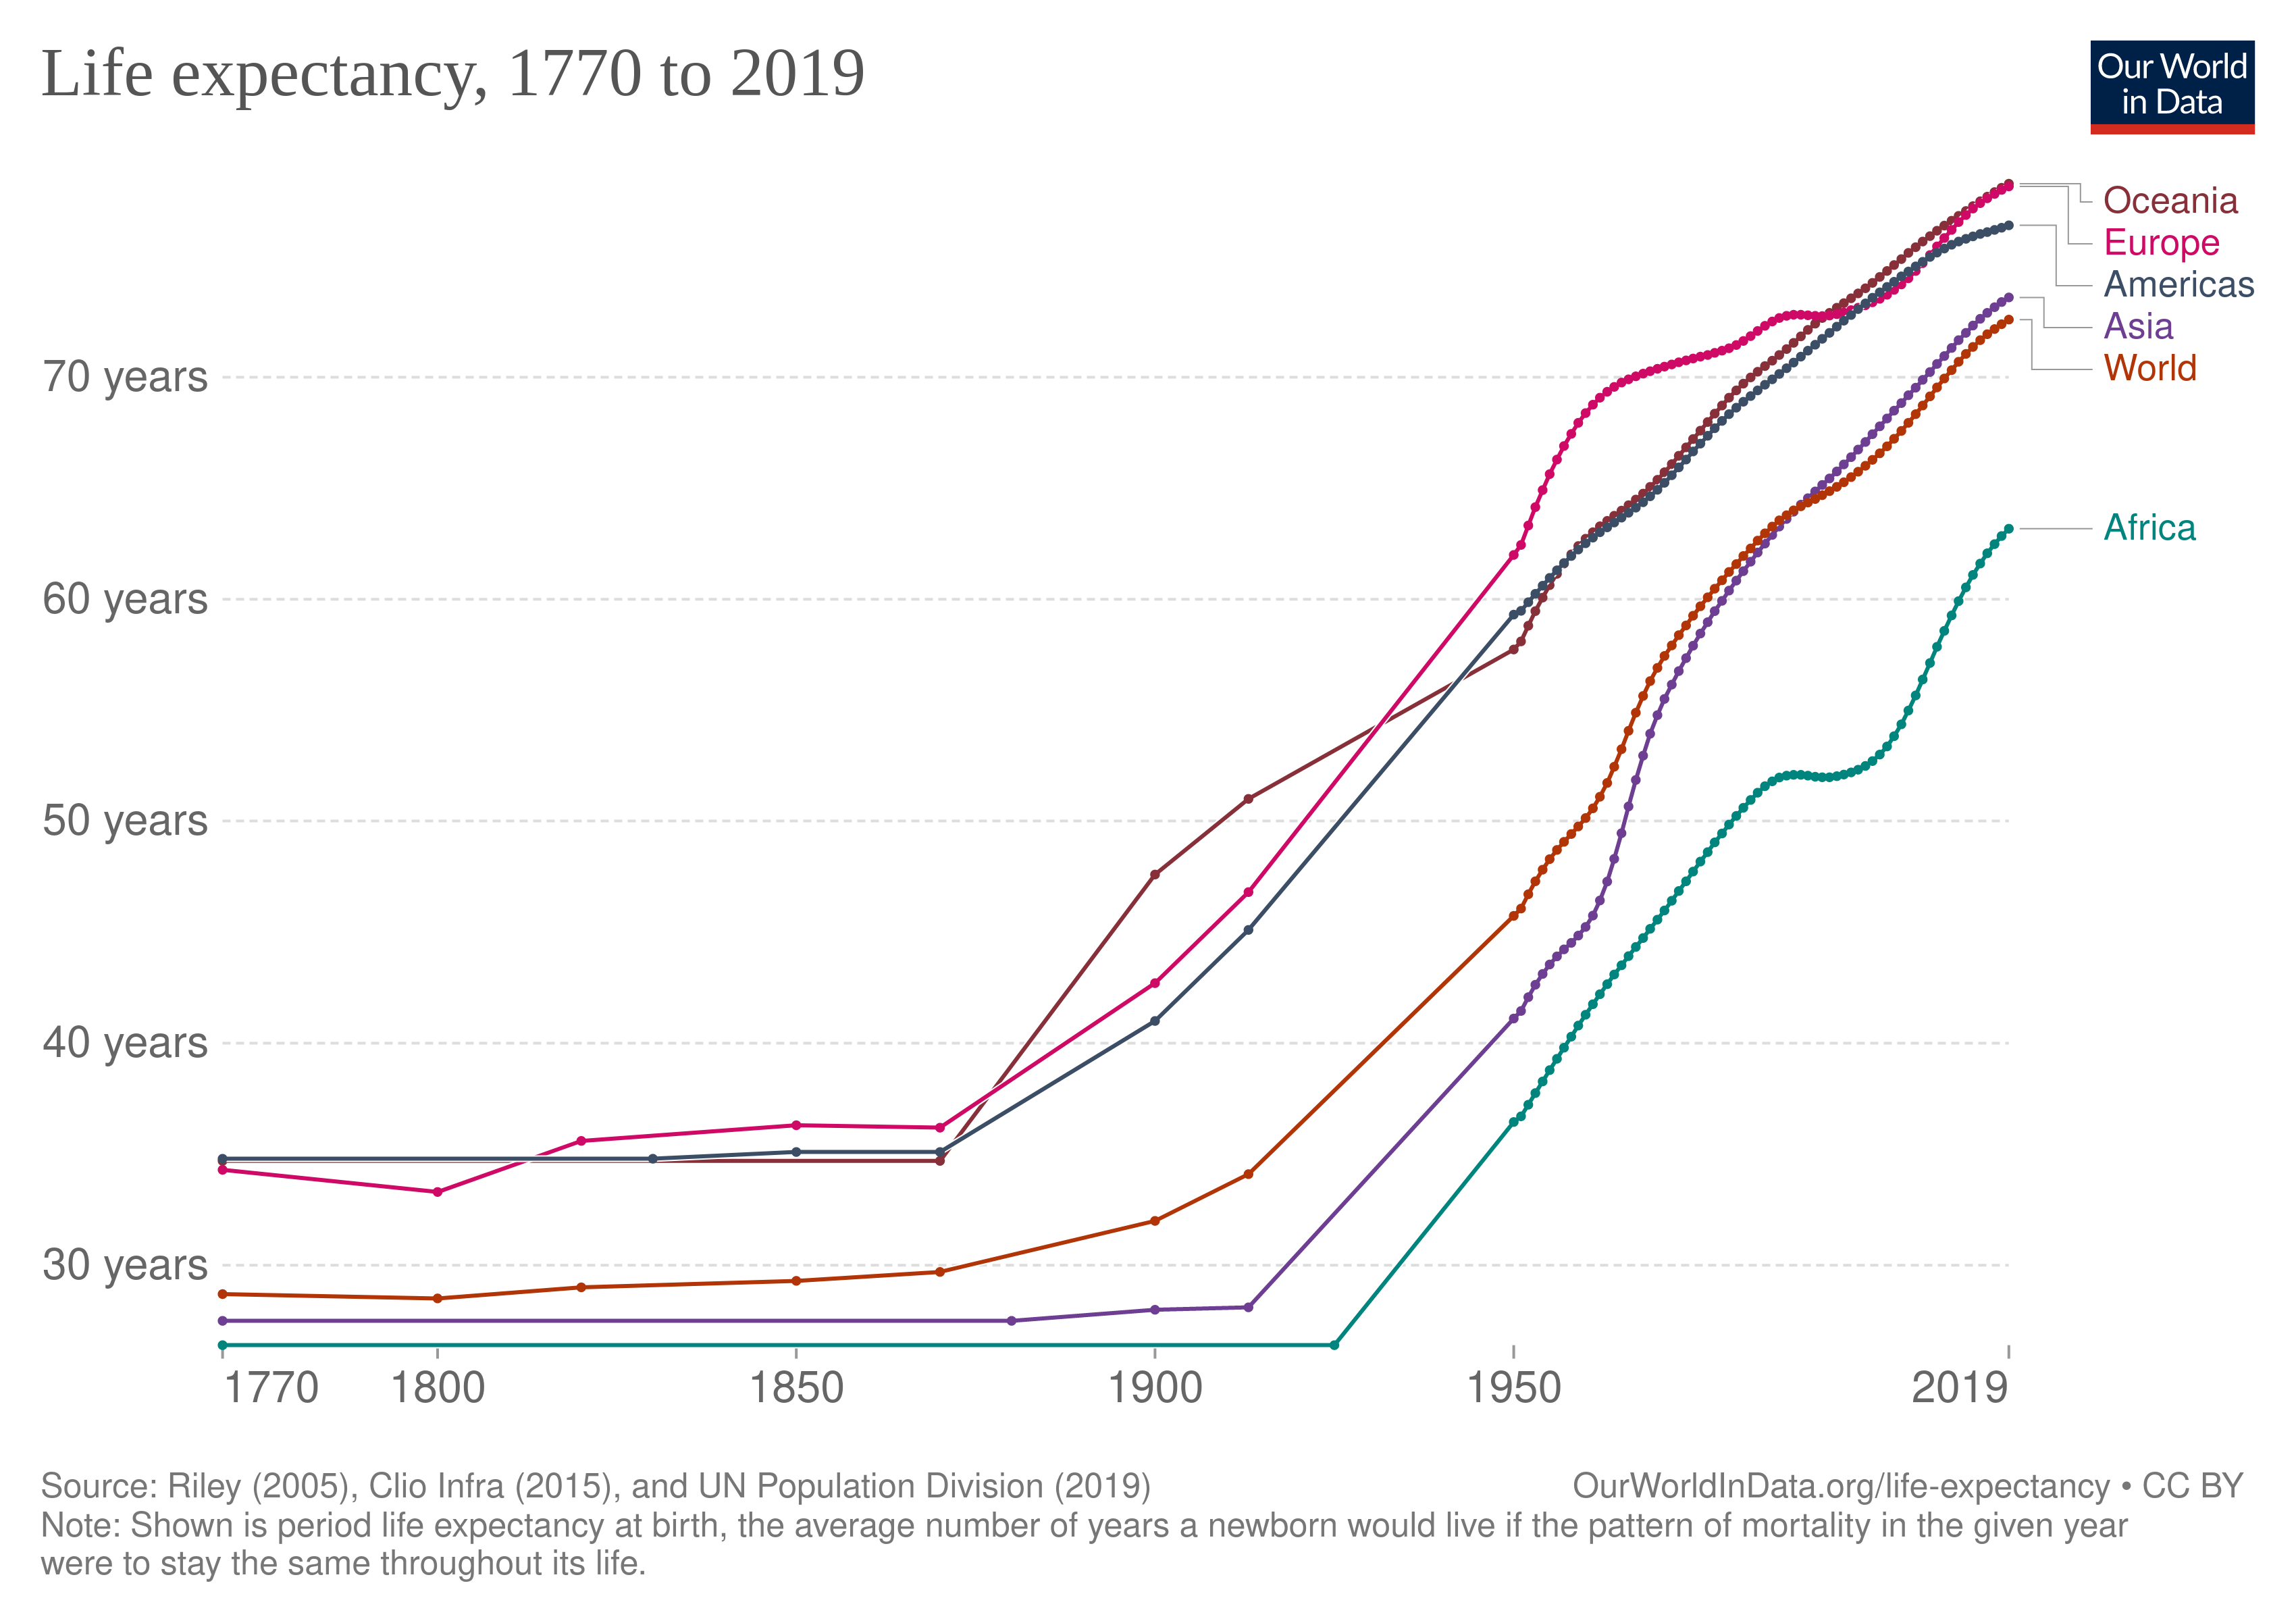
\includegraphics[width=12cm]{figures/life-expectancy}
  \caption {Очаквана продължителност на живота за различни региони през периода 1770-2019 \cite{zijdeman2016}.}
  \label{fig:life_expectancy}
\end{figure}

\paragraph{}
Застаряването на населението оказва неблагоприятен ефект и върху икономиката на държавите. Първо, заради увеличаването на дяла на хора, които не участват в работната сила. Второ, защото здравните системи ще бъдат допълнително натоварени с по-голям брой хора в напреднала възраст, за които рисковете от хронични заболявания са значително по-големи. Например, разходите за лечение на Алцхаймер възлизат на 305 милиарда щатски долара годишно, като се очаква със застаряването на населението тези разходи да достигнат над 1 трилион щатски долара \cite{wong2020}. Разходите за третиране на диабет се очаква да достигнат над 2 трилиона долара до 2030 година \cite{bommer2018}.

\section[Молекулярно-биологични основи на живата материя]{Молекулярно-биологични основи на\\ живата материя}\label{sec:basic_genetics}

\paragraph{}
Стареенето е универсален процес, който се наблюдава при всички живи същества. Темповете на остаряване до известна степен имат индивидуални разлики, но са сравнително хомогенни сред всички представители на определен вид. Това подсказва, че съществуват генетични и наследствени фактори, които определят продължителността на живота, както съществуват такива фактори, които определят различни други фенотипни характеристики. Систематичното изследване на наследствеността започва през 19-ти век с работата на Грегор Мендел, който изучава научно моделите по които определени характеристики биват предавани от едно поколение на друго. Следващите поколения учени откриват, че съхраняването и изразяването на генетичната информация има забележителни сходства във всички познати форми на живот.

\paragraph{}
Сред всички познати видове, генетичната информация се съдържа в две разновидности на нуклеиновата киселина - рибонуклеинова киселина (РНК) и дезоксирибонуклеинова киселина (ДНК) \cite{houlihan2017}. ДНК представлява полимер, съставен от две полинуклеотидни вериги, навити една около друга, така че да образуват двойноспираловидна структура. Полинуклеотидните вериги са създадени от последователности от мономери - нуклеотидни бази. В състава на ДНК се включват четири вида бази - аденин (А), цитозин (C), гуанин (G) и тимин (T). Базите A и T образуват двойки помежду си, както и базите C и G. Казваме, че двете полинуклеотидни вериги на ДНК са комплементарни. Всеки ген може да бъде разположен на коя да е от двете вериги на ДНК и се описва от дълга последователност от нуклеотидни бази \cite[стр. 301-310]{klug2014}. PНК молекулата представлява единична полинуклеотидна верига, като вместо тимин (T) се използва урацил (U). РНК молекулата е химически по-реактивна от ДНК и по-нестабилна \cite{soukup1999}\cite{cristescu2019}. Поради тази причина, извън вирусите, РНК молекулата рядко се използва за дълготрайно съхранение на генетична информация и служи в други роли, като спомага при копирането на генетичната информация от ДНК (транскрипция) и превеждането ѝ в протеин (транслация).

\paragraph{}
Догмата в молекулярната биология представя основния път за реализация на генетичната информация в посоката ген-РНК-протеин \cite{crick1970central}. Първата стъпка към това е транскрипцията, при която ензимът РНК-полимераза копира информацията от ДНК в комплементарна РНК молекула \cite{sims2004}. За целта, РНК-полимеразата се свързва с определен участък преди началото на гена, наречен промоторен участък. Следва процеса на елонгация, при който ензимът се плъзга по шаблонната ДНК нишка и удължава РНК молекулата, като съпоставя комплементарна нуклеотидна база за всяка база от шаблонната нишка. При достигане на участък наречен терминатор, процесът приключва и РНК-полимеразата, първичната РНК молекула и ДНК нишката се отделят една от друга.

\paragraph{}
След транскрипцията първичната РНК молекула (pre-mRNA) преминава прецес на сплайсване, при който части от нея (интрони) биват изрязвани и остранени. Останалите части (екзони) се снаждат отново. Този процес се осъществява от комплекс от протеини, наречен сплайсозом. Първичната РНК може да бъде сплайсната по алтернативни начини, което дава възможност за образуването на голям брой различни протеинови изоформи от малък брой гени \cite{stamm2005}. Между 40\% и 60\% от човешките гени имат алтернативни сплайсови форми \cite{modrek2002}. След сплайсването си, първичната РНК молекула е трансформирана в зряла матрична РНК (мРНК/mRNA), и се изнася чрез активен транспорт от ядрото в цитоплазмата \cite{siebrasse2012}.

\paragraph{}
Зрялата мРНК, бива транспортирана до рибозомите, където генетичната информация, която тя пренася бива използвана за да се синтезира протеин. Рибозомата синтезира протеина, като на всеки кодон (група от три нуклеотидни бази) от мРНК молекулата се съпоставя определена амино-киселина (виж фиг. \ref{fig:transcription_splicing_translation}). Верига от амино-киселини образува протеин \cite[стр. 412-420]{klug2014}.

\begin{figure}[htp]
  \centering
  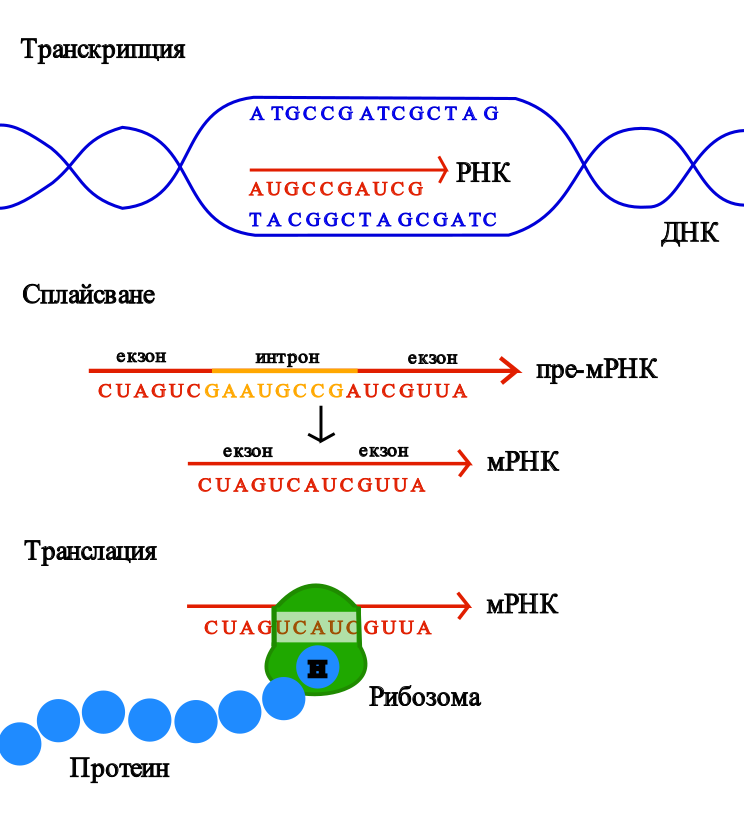
\includegraphics[width=12cm]{figures/transcription_splicing_translation}
  \caption {Графична репрезентация на процесите на транскрипция, сплайсване и транслация. Транскрипция е процесът на копиране на генетичната информация от ДНК молекулата в първична РНК молекула. Сплайсването е пост-транскрипционна модификация, при която се изрязват региони, наречени интрони, като е възможно алтернативно сплайсване на ген, позволяващо кодирането на множество протеини от един ген. Транслация е процесът, при който спрямо кода в зрялата мРНК молекула се синтезира протеин.}
  \label{fig:transcription_splicing_translation}
\end{figure}

\section[Молекулярно-биологични характеристики на стареенето]{Молекулярно-биологични характеристики\\ на стареенето}
\paragraph{}
Стареенето е въпрос, който вълнува учените от дълго време. През 1990-та, Медведев твърди, че вече съществуват над 300 теории за стареенето \cite{medvedev1990}. Въпреки постигнатият значителен прогрес през последните години в областта на геронтологията, причините за стареенето все още оставан ненапълно обяснени. Това се дължи на факта, че стареенето е сложен процес, в който са намесени множество фактори. Все още липсва голяма обединяваща теория на стареенето, която да обясни изцяло процеса, но съществуват множество теории, които дават добра представа за различни негови аспекти \cite{vina2007}. Следват основните биологични характеристики, които тези теории засягат (фиг. \ref{fig:biological_characteristics_of_aging}):

\begin{figure}[htp]
  \centering
  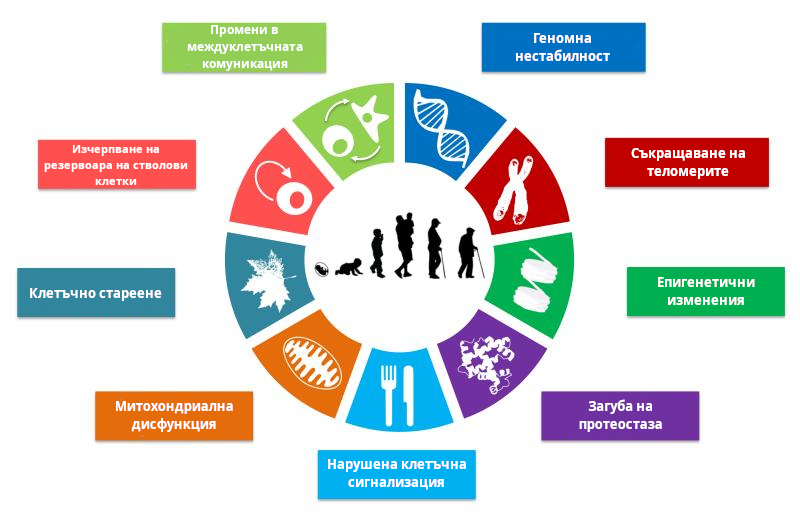
\includegraphics[width=15cm]{figures/biological_characteristics_of_aging}
  \caption {Основните биологични характеристики на стареенето. Източник на фигурата са Лопез-Отин и колеги \cite{lopezotin2013}, като фигурата е преведена на български.}
  \label{fig:biological_characteristics_of_aging}
\end{figure}

\subsection{Натрупване на геномни изменения}
\paragraph{}
Изменения в ДНК молекулите могат да настъпят както в следствие на вътрешноклетъчни фактори, така и поради въздействието на външни мутагени. Примери за вътрешноклетъчни фактори са случайни грешки при репликация и оксидативния стрес, предизвикан от натрупването на свободни радикали \cite{wang1998}. Външните мутагени могат да бъдат разделени на три вида - физични, химични и биологични. Пример за физичен мутаген е радиацията \cite{breimer1988}, a за биологичен вирусните инфекции, които също могат да предизвикат генетични мутации. Измененията в ДНК молекулите включват различни видове мутации като точкови мутации, делеции и инсерции, транслокации, инверсии и др.\\\\
Съществуват механизми, чрез които клетките засичат мутациите и ги поправят. Основни такива механизми са гените ATM и TP53. Все пак, тези механизми не са ефективни на 100\% и ефективността им допълнително спада с възрастта \cite{auley2017}. В резултат, в течение на времето, ДНК молекулите акумулират все повече мутации. Смята се, че тази геномна нестабилност е един от основните фактори, допринасящи за процеса на стареенето \cite{vijg2013}.

\subsection{Съкращаване на теломерите}
\paragraph{}
Теломерите са регион, намиращ се в края на хромозомите, в който се съдържат повтарящи се поредици от нуклеотидни бази. Те служат за предпазване на хромозомата от рекомбинация и постепенна деградация и дават възможност на клетката да различава края на хромозомата от случайни прекъсвания, при които биха били активирани механизмите за поправка на ДНК \cite{griffith1999}. При всеки цикъл на делене на клетката, теломерите се скъсяват поради непълното синтезиране на изоставащата нишка от ДНК полимеразата \cite{koliada2015}. Този проблем се компенсира донякъде от ензима теломераза, който пренася своя собствена РНК молекула и я използва като шаблон, спрямо който да удължи скъсения теломер. Въпреки това, недостатъчната експресия на теломеразата води до постепенното скъсяване на теломерите. Това може да доведе до загуба на репликативна способност на клетката и блокирането на клетъчния ѝ цикъл, процес известен като клетъчно стареене \cite{muraki2012}. Установено е, че първоначалната дължина на теломерите няма връзка със стареенето при различни видове, но скоростта на тяхното скъсяване има значителна корелация със продължителността на живота им \cite{whittemore2019}.

\subsection{Клетъчно стареене}
\paragraph{}
През 1961 Хейфлик и Муурхед показват, че клетки отглеждани в култура имат ограничен капацитет за клетъчно делене \cite{hayflick1961serial}. Процесът на загуба на репродуктивни способности и спирането на клетъчния цикъл е известен като клетъчно стареене (cellular senescence). Клетъчното стареене може да настъпи в следствие от различни вътрешни и външни фактори, включително скъсяване или дисфункция на теломерите, онкогенеза или увреждане на ДНК \cite{micco2021}. Така, клетъчното стареене има важна роля за потискането на развитието на тумори като прекратява размножаването на раковите клетки \cite{jeyapalan2008}. Същевременно обаче, загубата на способност за делене на клетките, която е критична за замяната на увредените клетки и обновяването на тъкъните, дава основание да предположим, че клетъчното стареене може да има роля и в процеса на стареене на организма. Тази хипотеза се подкрепя и от in vivo изследвания, които показват, че с напредъка на възрастта се наблюдава натрупване на остарели клетки \cite{jeyapalan2008}. Асоциативни-изследвания върху целия геном (Genome Wide Association Studies или GWAS) пък са открили, че локуса \textit{INK4/ARF}, кодиращ свързани с клетъчното стареене протеини, има силна асоциация с множество свързани с възрастта заболявания като рак, синдром на Алцхаймер, старческа немощ и др \cite{jeck2012meta}.

\subsection{Епигенетични изменения}
\paragraph{}
Епигенетичните изменения са промени в активността и изразяването на гените без да се променя ДНК секвенцията. Някои епигентични промени са обратими, докато други се унаследяват и се обозначават като епигенетична наследственост. Епигенетичните промени имат ключова роля за запазването на стабилността на генома и осигуряват правилното развитие на индивида \cite{dupont2009}. Примери за епигентични промени са ДНК метилирането и хистоновите модификации. И за двете се смята, че са значими фактори в процеса на стареенето \cite{daquila2013}\cite{aitbaev2019}.

\paragraph{}
ДНК метилирането представлява добавяне на метилови групи към базите цитозин или аденин в ДНК молекулата, като една от основните му роли е да потиска транскрипцията на гени. С напредването на възрастта се наблюдава понижаване на нивата на общото ДНК метилиране, с изключение на някои специфични региони, при които нивото се повишава \cite{jung2015}.

\paragraph{}
Хистоните имат важна структурна роля при организирането на човешкия геном в хроматин. Основната изграждаща единица на хроматина е нуклеозомът, който представлява 147 базови двойки от ДНК увити 1.65 пъти около хистонов октамер. Връзката между хистоните и ДНК молекулата не позволяват на ензима РНК полимераза да достъпи ДНК молекулата и блокират транскрипцията. Този проблем бива преодолян от група протеини и ензими, които се грижат за отделянето на хистоните от ДНК молекулата и последващото им свързване \cite{das2012}. Метилирането на хистоните може да доведе както до активация на транскрипцията, така и до потискането й, в зависимост от хистона, метилираната аминокиселина и нивата на метилиране \cite{yi2020}.

\subsection{Загуба на протеостаза}
\paragraph{}
Всички клетки поддържат своята протеинова хомеостаза или протеостаза чрез прецизно координирани системи, които бързо коригират нежеланите протеомни промени \cite{kaushik2015}. За целта, неправилно нагънатите протеини биват поправяни или, ако това е невъзможно, деградирани и отстранени напълно. Стареенето, както и някои свързани с него заболявания, се свързват с нарушена способност за запазавне на протеостазата в клетките \cite{lopezotin2013}.

\subsection{Нарушена клетъчна сигнализация}
\paragraph{}
Изследвания на моделни организми показват, че генетични мутации, понижаващи активността на клетъчната сигнализация за наличие на хранителни вещества, могат да доведат до значително удължаване на продължителността на живота. Понижаването на активността на тези сигнални пътища води до подобно физиологично състояние като това при естествени периоди на недостиг на храна в природата. Известно е, че ограничаването на храненето (намаляване на приема на храна без недохранване) удължава средната и/или максималната продължителност на живота на различни организми, включително дрожди, мухи, червеи, риби, гризачи и макаци резус \cite{fontana2010}.

\subsection{Митохондриална дисфункция}
\paragraph{}
С напредването на възрастта, при бозайниците се натрупват соматични мутации на митохондриалната ДНК (мтДНК), водещи до намаляването на функцията на дихателната верига и влошаване на митохондриалната функция \cite{trifunovic2008}. Множество изследвания \cite{kujoth2005}\cite{vermulst2008} показват, че митохондриалната дисфункция води до ускорено стареене и настъпване на редица физиологични промени, свързани с възрастта, като например загуба на тегло, намаляване на подкожната мастна тъкан, алопеция (косопад), кифоза (изкривяване на гръбначния стълб), остеопороза, анемия, намалена плодовитост и уголемяване на сърцето \cite{trifunovic2008}.

\subsection{Изчерпване на резервоара на стволови клетки}
\paragraph{}
Изследвания показват, че стареенето може да се дължи отчасти и на изчерпването на стволовите клетки, които имат ключова роля в обновяването на тъканите. Потенциалните причини за изчерпването на стволовите клетки са многобройни, но общоприета е теорията, че тези клетки се губят в резултат на естествено възникващи мутации и увреждания на ДНК, които водят до клетъчна смърт \cite{ruzankina2007}\cite{revuelta2017}.

\subsection{Промени в междуклетъчната комуникация}
\paragraph{}
Освен промени в отделните клетки, стареенето включва и промени на ниво междуклетъчна комуникация \cite{lopezotin2013}. Дерегулацията на междуклетъчната комуникация може да доведе до редица негативни последици, като например хронични възпаления, нарушена функция на имунната система, увеличаване на свързания със стареенето секреторен фенотип (Senescence-Associated Secretory Phenotype), промени в комуникацията на ендокринната и невронната системи и други \cite{lagger2021}.

\section[Генетични фактори, влияещи на процеса на стареене]{Генетични фактори, влияещи на процеса\\ на стареене}
\paragraph{}
В секция 2.2.2 беше представен кратък обзор на различните биологични процеси, които способстват процеса на стареене. Предвид, че тези процеси също биват контролирани от действието на определени гени \cite{liu2004}\cite{jin2018}\cite{tominaga2002}, уместно е да предположим, че промени в тези гени могат да повлияят и на процеса на стареене като цяло, както положително така и отрицателно. Има множество примери за това, съществуващи в научната литература, като голяма част от тях са събрани в публичната база данни Human Ageing Genomic Resources (HAGR), която представлява колекция от ресурси за изследването на стареенето при хората. Някои записи в HAGR са включени на база установена директна връзка между даден ген и стареенето, докато други са включени на база ролята на гена в различни човешки патологии. Много от записите са подбрани, тъй като за техни хомолози в други организми е била открита връзка със стареенето. Към момента в HAGR са налични над 300 човешки гена, за които се предполага, че имат потенциална връзка със стареенето \cite{tacutu2018}.

\subsection[Видове генетични варианти]{Видове генетични варианти}
\paragraph{}
Съществуват различни видове генетични варианти, като например точкови мутаци, вмъквания, изтривания, инверсии, дублирания и др. Ефектът им може да варира от никакъв до инактивиране на жизненоважни гени \cite{taiping1998}. Мутациите могат да засегнат както протеин-кодиращи региони в генома, така и интрони или региони между гени, като дори мутации в междугенните региони могат да имат значително въздействие \cite{zou2020}.

\subsubsection{Точкови мутации}
\paragraph{}
Точковата мутация представлява замяна на една нуклеотидна база от референтния геном с друга. Това е най-често срещания тип генетични варианти, като типичния геном съдържа между 3.5 и 4.3 милиона точкови мутации . Заедно с кратките вмъквания и изтривания, точковите мутации съставляват около 99,9\% от всички генетични варианти \cite{auton2015}. В зависимост от ефекта, който варианта има върху кодирания протеин, се делят на няколко вида (фиг. \ref{fig:snp_types}).

\begin{figure}[h]
  \centering
  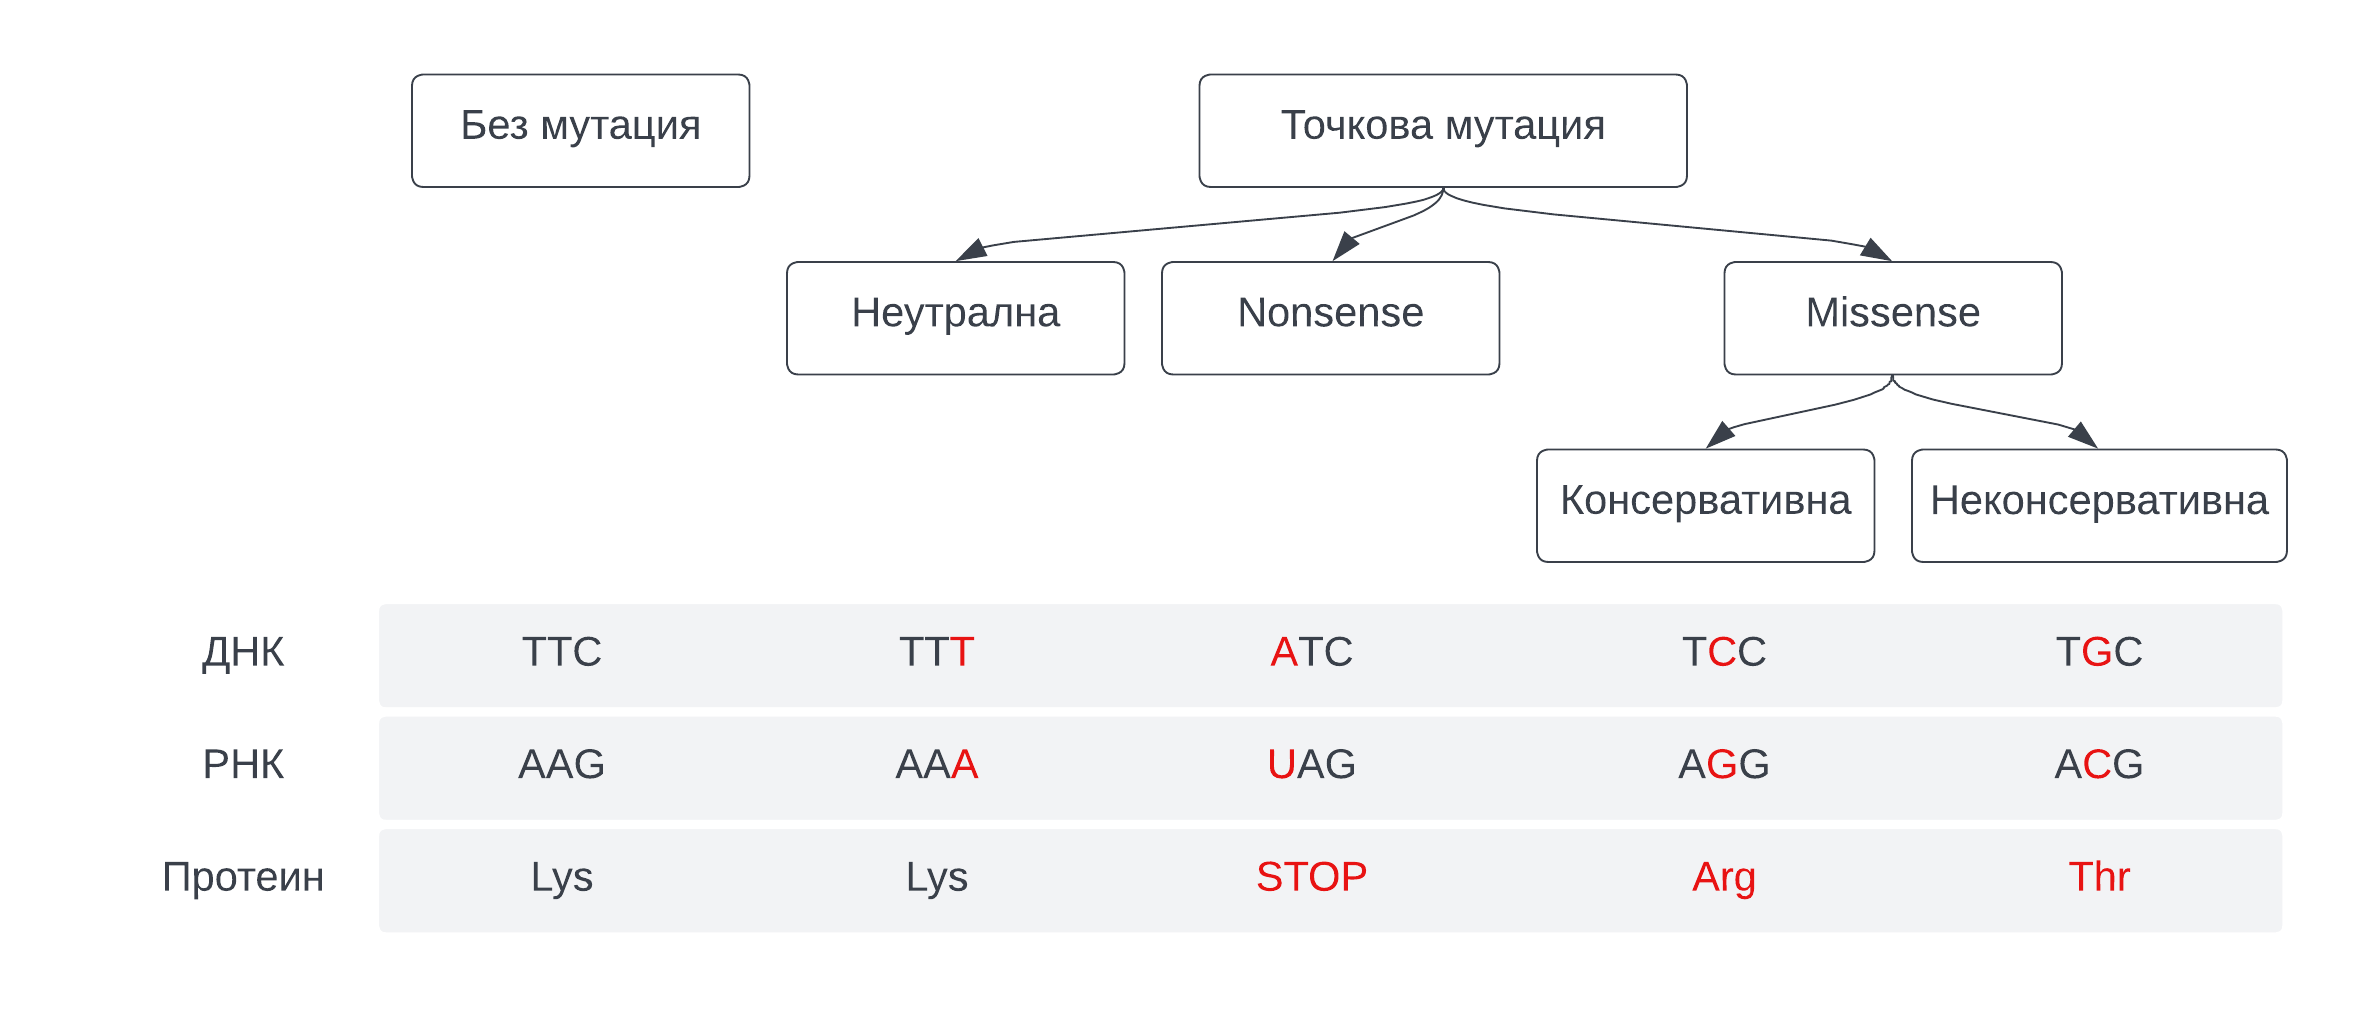
\includegraphics[width=17cm]{figures/snp_types}
  \caption {Различни видове точкови мутации и примери за тях.}
  \label{fig:snp_types}
\end{figure}

\paragraph{}
Неутралните (synonimous) мутации променят кодона към друг, който кодира същата аминокиселина. Такива мутации обикновено не се очаква да променят фенотипа, но съществуват и изключения \cite{kimchi2007}. Nonsense мутациите, заменят кодона с такъв, който води до прекратяване на транслацията. Това създава частичен протеин, който може да загуби функция си \cite{bidou2012}. Missense мутациите водят до промяна на аминокиселината, която кодона кодира. Ако новата аминокиселина има сходни свойства с референтната, мутацията се нарича консервативна, а иначе неконсервативна.

\paragraph{}
Пример за точкова мутация, която се асоциира със стареенето, е вариантът Rs2075650 в гена \textit{APOE}, кодиращ протеина Аполипопротеин Е, който има роля в метаболизма на мазнини \cite{deelen2011}\cite{lu2014}.

\subsubsection{Вмъквания и изтривания}
\paragraph{}
Вмъкванията и изтриванията представляват добавяне или премахване на между 1 и 10000 нуклеотидни бази от генома на организъм \cite{mullaney2010}. Те представляват вторите най-разпространени генетични варианти, като всеки човек има средно 550-625 хиляди такива полиморфизми в генома си \cite{auton2015}. Ако дължината на вмъкването или изтриването не е кратна на три, вариантът създава frameshift мутация (мутация с изместване на рамката на четене). Това може да промени до голяма степен секвенцията на кодирания протеин от мутацията до края на протеина или до следващата frameshift мутация, която да възвърне оригиналната рамка. Вмъквания и изтривания, предизвикващи изместване на рамката на четене са редки в кодиращите части от генома, но се срещат често в некодиращите региони \cite{bai2013}.

\subsubsection{Други}
\paragraph{}
Съществуват и множество други, по-големи структурни мутации, които са по-редки, но обхващат по-голям брой нуклеотидни бази \cite{auton2015}. Те включват големи изтривания (10000 или повече бази), промяната на броя на копията на дадена последователност, инверсии и други.

\section{Биоинформатика}
\paragraph{}
Количеството данни, което се генерира в областта на биологическите науки, през последните години бележи забележителен ръст \cite{marx2013}. Например, Европейския институт по биоинформатика през 2020 година отчита, че съхранява 390 петабайта данни \cite{embl2021}. За работа с подобно количество информация се нуждаем от помощта на компютърни системи. Тук се явява и важната роля на биоинформатиката, която представлява науката за прилагането на компютърно-изчислителни техники за обработка на информация свързана с биомолекули \cite{luscombe2001}.

\paragraph{}
Биоинформатиката има три основни цели \cite{luscombe2001}. Първата е съхраняването на големите обеми от данни по начин, който дава възможност на изследователите да намират и достъпват наличната информация, както и да добавят нова такава. Втората цел е разработката на инструменти и ресурси, които да спомагат за анализа на данни. Третата цел е използването на тези инструменти за анализа и интерпретацията на данни, с цел отговор на някакъв биологически въпрос.

\paragraph{}
Биоинформатиката намира приложение в изключително много аспекти от съвременните биологически изследвания. Съвременните техники за геномно секвениране (Next-Generation Sequencing) разчитат на различни биоинформатични техники за всички стъпки от процеса: от анализ на сигналите и разпознаване на нуклеотидните бази, подравняването на сегменти спрямо референтен геном, до асемблирането на цялостен геном \cite{oliver2015}. След като геномът е секвениран, той трябва да бъде анотиран, за да се добавят връзките между определени геномни региони и биологическите им функции \cite{aken2016}. За тази цел, също могат да се изполват автоматизирани биоинформатични решения \cite{curwen2004}. Други примери за области, където се прилагат биоинформатични техники са, например, асоциативни изследвания, търсещи статистически връзка между генетични варианти и определни фенотипи \cite{moore2010}, предсказване на триизмерната структура на протеини \cite{alphafold2021}, откриване на лекарства \cite{searls2000}, изследване на еволюционното развитие на видове \cite{diniz2017} и други.

\section[Значение на биоинформатиката за изследването на стареенето]{Значение на биоинформатиката за\\ изследването на стареенето}
\paragraph{}
Изучаването на стареенето при хората среща две големи затруднения. Първото е сложността на фенотипа на стареенето и множеството различни изменения в организма, настъпващи с остаряването. Второто е трудността на провеждане на \textit{in vivo} изследвания на хора, които също така имат сравнително голяма продължителност на живота. Поради тези причини, много изследователи на стареенето използват различни моделни организми за своите изследвания. При някои видове, като например мишките и приматите, се наблюдава забележително генетично сходство с хората и подобни фенотипи на стареенето, което често, обаче, има много различна скорост. За да разберем причините за тези разлики, днешните технологии ни дават възможност за генерирането на големи количества данни, които могат да бъдат анализирани посредством различни биоинформатични техники. Такива са сравнителния геномен анализ, филогенетичния footprinting (отпечатване), използването на ДНК микрочипове за намиране на нивата на експресия на гени, \textit{in silico} методи за моделиране на генрегулаторни мрежи и други \cite{demagalhaes2004}.
 
\section[Обзор на съществуващи биоинформатични решения]{Обзор на съществуващи\\ биоинформатични решения}
\subsection{VCF файлове}
\paragraph{}
Variant Call Format (VCF) е стандартен файлов формат, който се използва за описване на генетичните полиморфизми за дадена секвенция (за примерен файл виж фиг. \ref{fig:example_vcf}). VCF е текстов файлов формат с разделители-табулации (tab-delimited), който често бива съхраняван в компресиран вид, с цел оптимизиране на хардурерните ресурси, като дори компресиран може да бъде индексиран за бързо търсене. Във VCF могат да бъдат описани различни видове полиморфизми, от прости като точкови мутации, инсерции и делеции до по-сложни като например инверсии. VCF може да съдържа коментари, заглавен ред и редове за данни. В редовете за данни, всеки ред показва един полиморфизъм, като обикновено се използват стандартни референтни геноми, спрямо които се определят полиморфизмите. Файловият формат позволява и добавянето на богата анотация и потребителски-дефинирани полета. VCF стандартът е разработен за 1000 Genomes Project, а впоследствие е добил широка приемственост в биоинформатичната общност \cite{danecek2011}.

\begin{figure}[h]
  \centering
  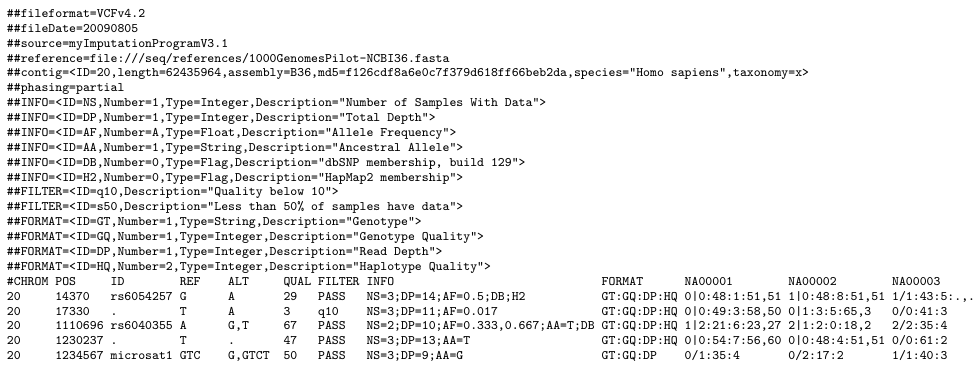
\includegraphics[width=17cm]{figures/vcf}
  \caption {Примерен VCF файл}
  \label{fig:example_vcf}
\end{figure}


\subsection{Анотация на генетични варианти}
\paragraph{}
С напредъка на технологиите за секвениране способността за бързо генериране на големи обеми от данни за генетични варианти бързо расте. Същевременно се образува все по-голяма пропаст между възможностите за генериране на нови сурови данни и възможностите за извличане на полезна информация и познание от тях \cite{yang2015}. Основна стъпка за разбирането на суровите данни с генетични варианти е анотирането им. Анотацията представлява процес, при който към генетичните варианти се добавя допълнителна функционална информация \cite{mccarthy2014}. Това може да бъде информация към кои кодиращи секвенции и гени се отнася варианта, оценка на степента му на въздействие, индикация дали се променят аминокиселините на кодирания протеин \cite{cingolani2012}, предсказване на структурните и функционални промени в протеина \cite{mccarthy2014} и др.
\subsubsection{snpEff}
\paragraph{}
SnpEff е софтуер с отворен код, който може бързо да анотира и категоризира генни варианти на база на ефекта, който те биха имали върху анотираните гени. SnpEff поддържа анотацияа на различни видове полиморфизми, като например единични нуклеотидни полиморфизми (SNPs), множествени нуклеотидни полиморфизми (MNPs) и вмъквания-изтривания (Indels) \cite{cingolani2012}. SnpEff разполага с много богата база данни от различни референтни геноми, с които може да работи, а дава възможност на потребителя да използва и свой собствен референтен геном. Основният формат, с който SnpEff работи е VCF. След обработката на входния VCF файл, съдържащ по един полиморфизъм на ред, SnpEff добавя една или повече анотации за всеки полиморфизъм в полето INFO, като всяка анотация има ключ „ANN“. Някои от по-важните анотации, които SnpEff предоставя са: идентификация на генът, с който е свързан полиморфизма; идентификатори на транскриптите, които полиморфмизмът засяга; оценка на ефекта на полиморфизма и на промените, които би причинил в аминокиселинния състав на протеина, който кодира. SnpEff е имплементиран на програмния език Java, което го прави лесно преносим и му дава възможност да работи на изключително голям набор от операционни системи и устройства \cite[стр. 9-10]{schildt2020complete}.

\subsubsection{VEP}
\paragraph{}
Част от проекта Ensembl, VEP (Variant Effect Predictor) е иснтрумент за анализ и анотация на генетични варианти. Софтуерът е с отворен код, свободен за използване от всеки и поддържа пълна възпроизводимост на резултатите. VEP има разнообразни интерфейси. Той може да бъде достъпван като уеб услуга, чрез удобен потребителски интерфейс. Също така предоставя REST API, работещ със стандартния формат за сериализация JSON, което го прави удобен за интеграция с програми, независимо от използваните за тях програмен език и технологии. Възможно е и да бъде свален като Perl скрипт и използван локално, чрез командния ред на операционната система, като необходимите бази данни могат да бъдат кеширани също локално, за по-голямо бързодействие \cite{mclaren2016}. VEP анотациите съдържат разнообразна информация, включваща молекулярните последствия на варианта (което в snpEff наричат ефект), засегнатия ген и транскрипти, в кой екзон е полиморфизмът, определяне на промяната в аминокиселинния състав на протеина и оценка на въздействието \cite{hunt2022}.

\subsubsection{Annovar}
\paragraph{}
Annovar (ANNOtate VARiation) е програма за анотация и приоритизация на генетични варианти. Annovar е имплементиран на Perl и може да бъде свален и използван свободно за лични, научни и некомерсиални цели. Достъпна е и уеб версия, известна като wAnnovar (\url{https://wannovar.wglab.org/}). Annovar може да анотира варианти спрямо различни човешки референтни геноми, както и спрямо референтни геноми на различни видове моделни организми. Освен да анотира функционалните ефекти на генетични варианти, Annovar има и допълнителни функционалности. Възможно е анотиране спрямо геномни региони, различни от гени, като например ивестни добре запазени области от генома, предсказани участъци за прикрепяне на транскрипционни фактори, предсказани целеви участъци за микроРНК молекули и др. Annovar, също така, дава възможност за сравнение на варианти с вече известни такива, които са налични във външни бази данни \cite{wang2010}.

\subsection[Филтриране и анализ на генетични варианти]{Филтриране и анализ на генетични\\ варианти}
\subsubsection{snpSift}
\paragraph{}
SnpSift е софтуер за филтриране и промяна на VCF файлове, съдържащи анотирани генетични варианти. Чрез SnpSift могат да се извършат различни операции, като например филтриране по геномен регион, разделяне на файла по хромозома, извличане на определени полета, допълнително анотиране спрямо външни бази данни, както и филтриране с потребителски дефиниран логически израз. Филтрирането с потребителски израз работи посредством рекурсивна граматика, която може да обработва изрази с произволна сложност \cite{cingolani2012sift}. Това прави SnpSift доста мощен инструмент за лесна обработка и анализ на генетични варианти и извличане на информация от тях. SnpSift, също като SnpEff, е имплементиран на програмния език Java, което му дава голяма преносимост върху различни операционни системи и платформи \cite[стр. 9-10]{schildt2020complete}.

\subsubsection{bcftools}
\paragraph{}
Bcftools е програма, предлагаща множество команди за обработката и анализа на VCF файлове, компресирани VCF файлове и бинарния им еквивалент - BCF файлове. Програмата автоматично засича форматът на входните данни, без да е необходимо потребителят да го индикира. Една от командите на Bcftools е view. Тя дава възможност за филтриране и конвертиране на VCF и BCF файлове. При филтрирането могат да бъдат зададени голям набор от разнообразни критерии, като например по зададени геномни региони, тип на полиморфизма (точкова мутация, вмъквания-изтривания, и тн.), брой на алелите, и др. Възможно е и да се филтрира по булев израз, включващ кои да е полета от VCF файла \cite{danecek2021}.


\subsubsection{Cutevariant}
\paragraph{}
Cutevariant e програма с графичен потребителски интерфейс, която позволява филтрирането на генетични варианти заредени от вече анотиран VCF файл. Програмата поддържа файлове, анотирани със SnpEff или VEP. При зареждане на файл, програмата го обработва и записва информацията в SQLite база данни. Това позволява данните да бъдат филтрирани със сложни филтри, които могат да бъдат контролирани както посредством графичния потребителски интерфейс, така и посредством VQL - специален език, наподобяващ SQL \cite{schutz2021}.

\subsection{Геномни браузъри}
\paragraph{}
В последните години биологическите науки се превръщат в една от областите генериращи най-голямо количество данни \cite{Stephens2015}. Развитието на технологии за секвениране от ново поколене (next-generation sequencing или NGS) намалява цената и увеличава скоростта на секвенирането \cite{schuster2008}. В резултат, геномите на вече десетки хиляди организми са секвенирани и достъпни в онлайн бази данни, предоставящи информацията публично за свободно ползване \cite{mukherjee2020}. Освен секвенции, тези бази данни съдържат най-различни видове анотации, като например позициите на известни или предсказани гени, мРНК транскрипти, информация за генна експресия, генетични полиморфизми, сравнения с други организми, информация за епигенетични маркери, като нива на метилиране, и др.

\paragraph{}
Есенцията на геномните браузъри е представянето на различните видове данни като отделни информационни ленти една под друга, на които геномните координати са подравнени по вертикалната ос. По този начин потребителят може лесно да види дали има определени съвпадения, или разлики в информацията от различните ленти и да направи изводи за функцията или други характеристики на дадения геномен регион. Интеграцията на секвенции и богат набор от анотации прави геномните браузъри удобна платформа, чрез която молекулярните биолози могат да разглеждат, търсят, извеждат или анализират информация за генома ефективно и удобно \cite{wang2013brief}.

\subsubsection{UCSC Genome Browser}
\paragraph{}
На 22 юни 2000 година, UCSC (University of California, Santa Cruz) и другите членове на международния проект за секвениране на човешкия геном завършват първата работна версия на човешкия геном. Няколко седмици по-късно на 7 юли 2000 година, асемблирания геном става публично достъпен на уеб сайта на UCSC. Заедно с него става достъпен и графичен инструмент за разглеждането му - UCSC Genome Browser.

\paragraph{}
UCSC Genome Browser (фиг. \ref{fig:ucsc}) предоставя достъп и инструменти за разглеждане, сравняване и анализиране на геномите на голям набор от организми \cite{fujita2011}. Анотациите и информацията, представена от UCSC, идва от разнообразни източници, като GENCODE Genes, NCBI RefSeq Genes, Ensembl Genes и др \cite{navarro2021}. Също така, потребителят може да зареди анотации от свой собствен файл, като те се добавят като допълнителна информационна лента в браузъра. USCS Genome Browser предоставя прост графичен интерфейс, който дава възможност на потребителя да навигира из генома с функции като увеличаване и намаляване на резолюцията, преместване, търсене по ген, секвенция или геномна локация и др. При натискане върху обект, браузърът показва подробна информация за него. UCSC Genome Browser има възможност да зарежда и обработва огромни по обем файлове с анотации, без да престава да работи гладко \cite{kent2002human}. Браузърът поддържа разнообразни видове файлове, включително VCF \cite{navarro2021} и BAM \cite{fujita2011}. Достъпен е както онлайн, така и като самостоятелна програма.

\begin{figure}[h]
  \centering
  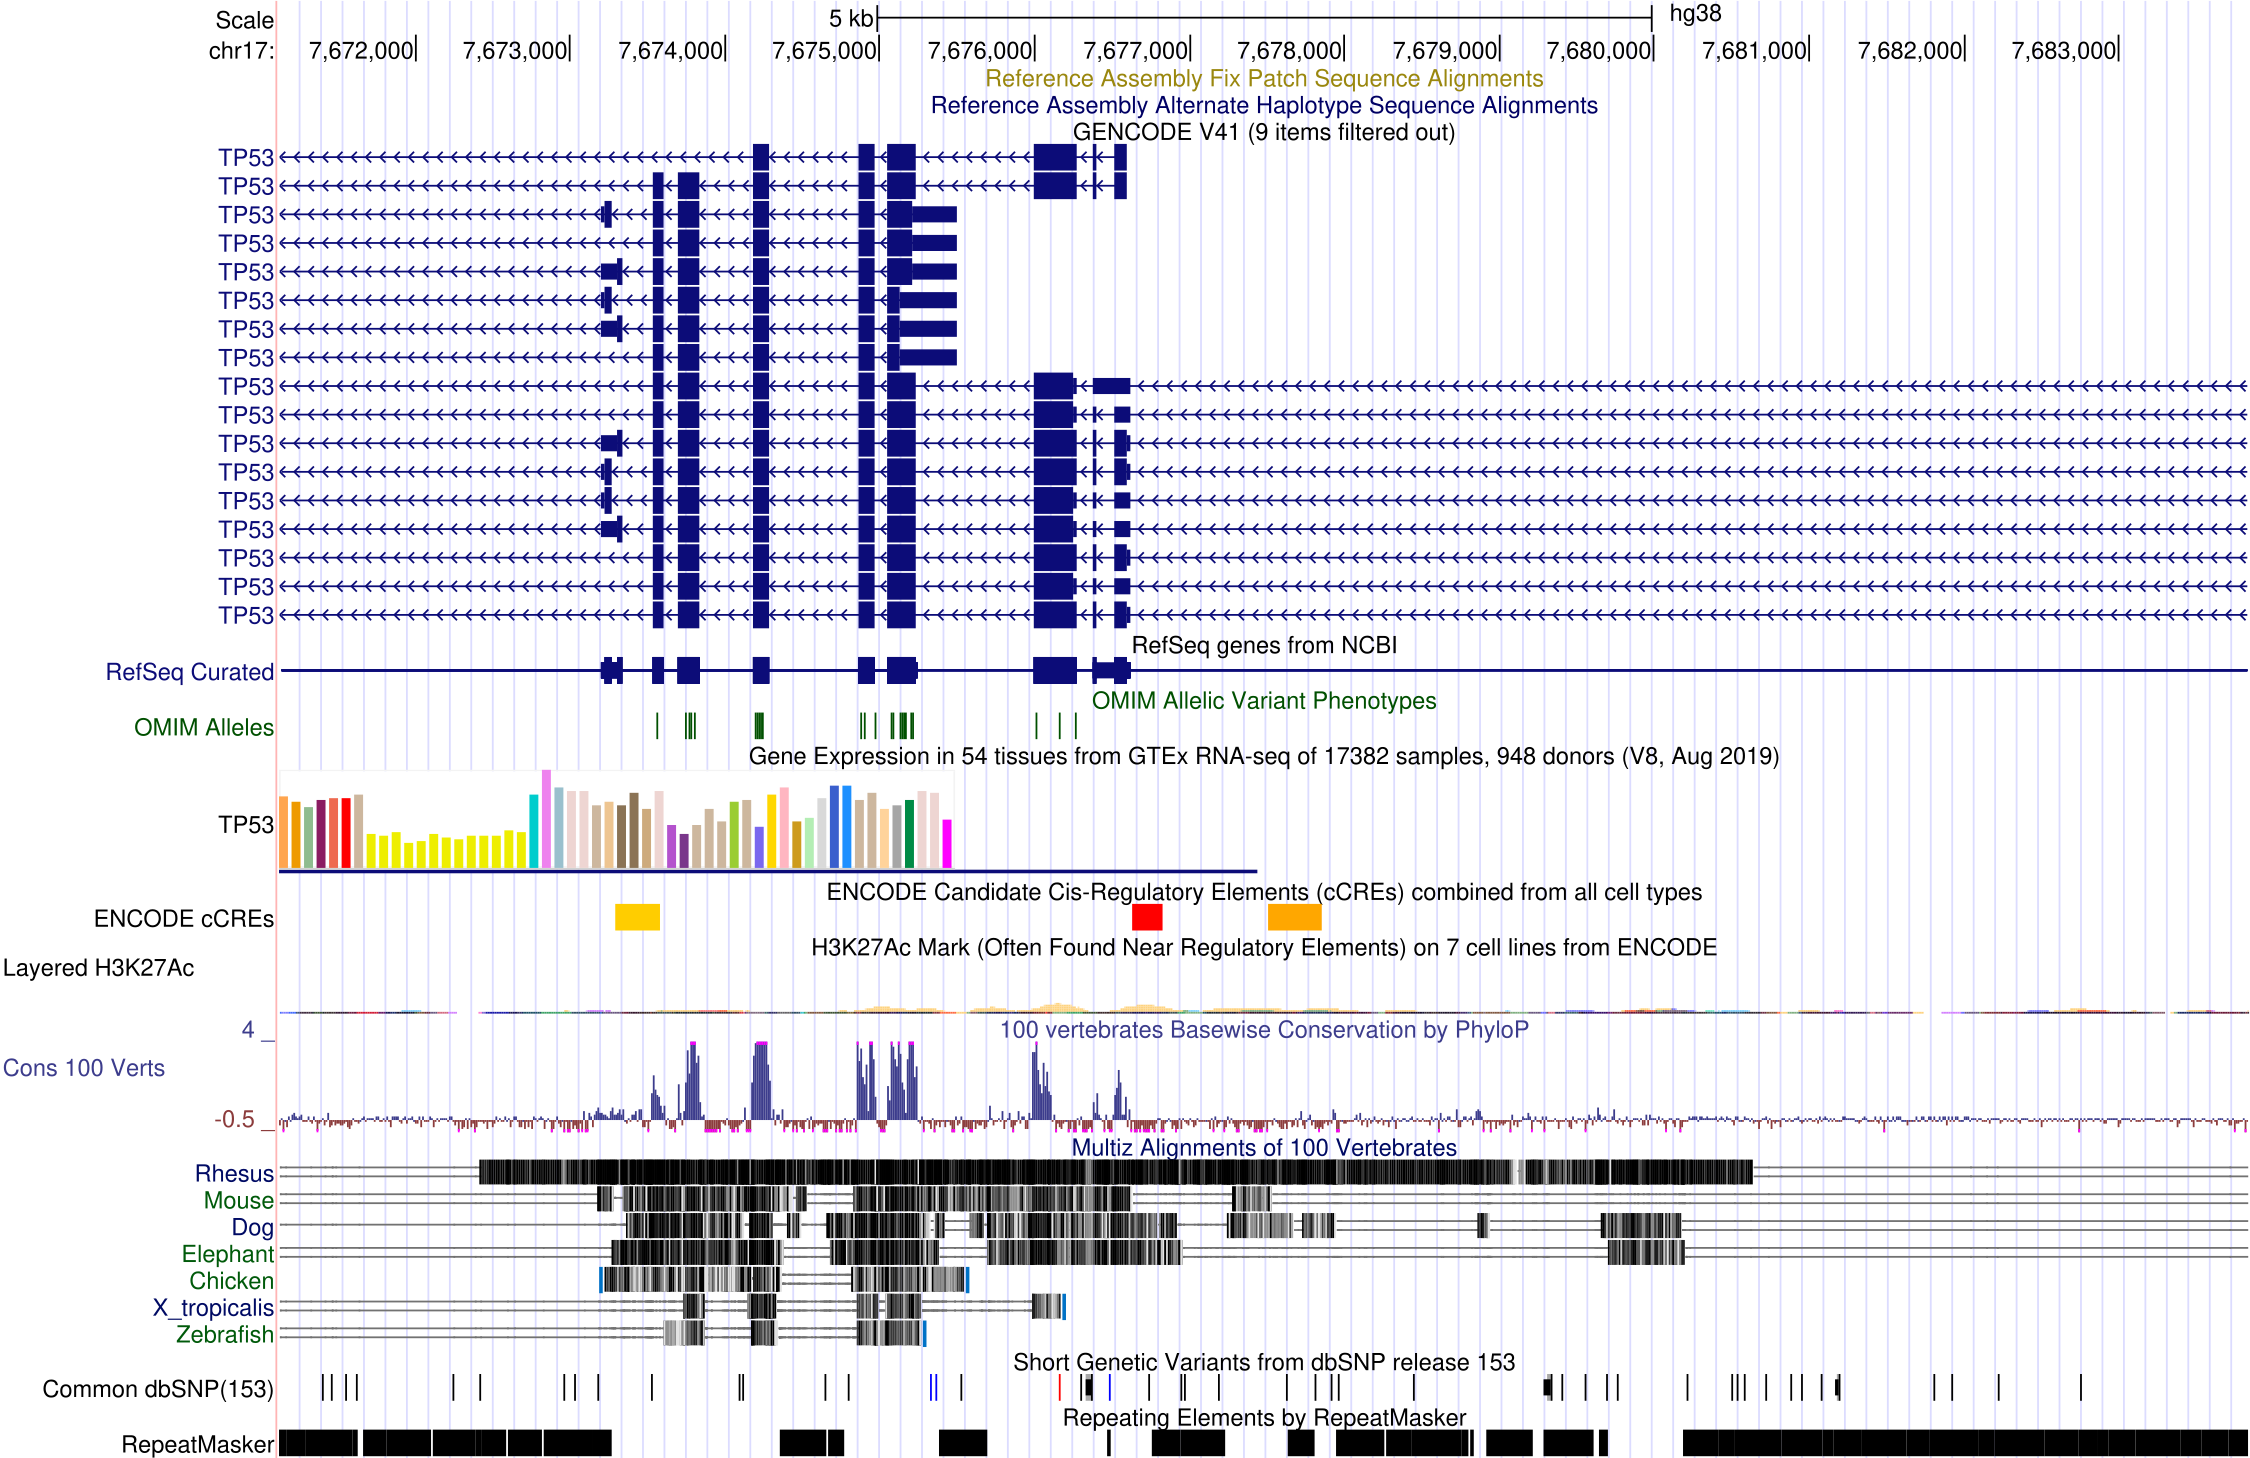
\includegraphics[width=16cm]{figures/UCSC}
  \caption {Примерна визуализация на генът TP53 с UCSC (http://genome.ucsc.edu).}
  \label{fig:ucsc}
\end{figure}

\subsubsection{IGV Genome Browser}\label{sec:igv}
\paragraph{}
IGV (Integrative Genomics Viewer) е инструмент за визуализация и интерактивно изследване на разнообразни, големи по обем геномни колекции от данни (фиг \ref{fig:igv_example}). Посредством IGV могат гъвкаво да се интегрират широк спектър от различни типове геномни данни, като например подравнени поредици, мутации, експресия на гени, метилиране, геномни анотации и др. IGV позволява на потребителя да изследва данните си на различни нива на резолюция, като дава възможност за приближаване и отдалечаване в реално време \cite{robinson2011}\cite{robinson2017}. Данните могат да бъдат зареждани както от публични онлайн бази данни, така и локално от данните, с които разполага потребителя.

\begin{figure}[h]
  \centering
  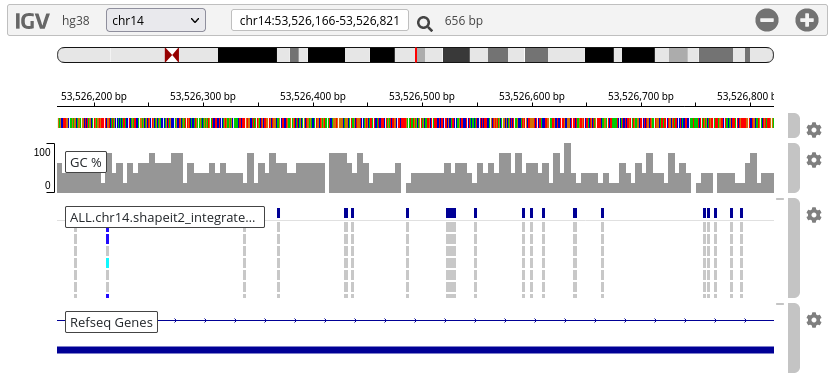
\includegraphics[width=17cm]{figures/igv_example}
  \caption {Примерна визуализация с IGV}
  \label{fig:igv_example}
\end{figure}

\paragraph{}
Едно от най-големите предимства на IGV е това, че лесно може да бъде интегриран във външна страница. Достатъчно е да бъде импортирана JavaScript библиотеката igv.js и да се извика функция за вграждане на геномния браузър в конкретен HTML елемент от страницата. IGV браузърът може да работи с различни файлови формати, като например FASTA, BAM и VCF. Може да поддържа големи обеми от данни, като за целта използва индексни файлове, на базата на които прави асинхронни заявки, за да вземе единствено частите от файла, които трябва да бъдат визуализирани. IGV може да се конфигурира и предоставя JavaScript API за взаимодействие между браузъра и съдържащото го приложение \cite{robinson2020}.

\subsection{Биоинформатични решения за определяне на 3D пространствена структура на протеини}
\paragraph{}
Протеините са макромолекули, които представляват дълга верига от аминокиселини. Протеините имат роля в множество процеси в организмите, като например катализирането на реакции, репликацията на ДНК, клетъчната комуникация, транспортирането на молекули, образуването на клетъчната структура и др. Както вече бе разгледано в секция \ref{sec:basic_genetics}, ДНК служи като шаблон за транскрипцията на мРНК молекули, които биват транслирани в протеини. По този начин генетичния код определя първичната структура на протеина, тоест последователността от аминокиселини. За да стана биологически активни, обаче, протеините трябва първо да заемат сгъната (третична) структура в пространството \cite{creighton1990protein}.

\paragraph{}
Триизмерната (третична) структура на протеина се определя от първичната му структура, тоест от последователността от аминокиселини. Движещи сили при нагъването на протеина са хидрофобните интеракции, образуването на междумолекулярни водородни връзки и силите на Ван дер Ваалс. Тези сили въздействат докато протеина не достигне оптимална и стабилна форма \cite{dill2008}. Откритието, че триизмерната структура на протеина зависи почти изцяло от последователността от аминокиселини, поражда търсенето на компютърен алгоритъм, който да може да предскаже триизмерната структура, която определена аминокиселинна поредица би образувала. В контекста на тази дипломна работа, ползата от такъв алгоритъм би била, че ако можем да покажем как определен генетичен вариант на ген, свързан със стареенето, би променил триизмерната структура на кодирания протеин, това би спомогнало за разбирането на това как генетичния вариант се отразява и на функцията му.

\subsubsection{Подходи}
\paragraph{}
Съществуват множество различни методи, които се опитват да решат проблема за предсказване на триизмерната протеинова структура. Те могат да бъдат разделени на четири групи: (1) такива, които се основават на базови принципи и не използват информация от външни бази данни; (2) такива, които се основават на базови принципи и използват информация от външни бази данни; (3) threading методи, при които аминокиселиината поредица се моделира спрямо множество от структурни-скелета, взети от готова библиотека с нагъвнания, като за всяко от тях се пресмята оценка за съвместимост; (4) сравнителни (или хомоложни) методи \cite{dorn2014}. Сравнителните методи се опитват да предскажат структурата на даден протеин като идентифицират подобни, вече известни, протеини и ги използват за шаблон, спрямо който да моделират структурата. При тези методи се разчита на наблюдението, че при хомоложните гени (гени, които си приличат поради обща еволюционна история) триизмерната структура на протеина е по-добре запазена от аминикиселинната му последователност \cite{illergard2009}.


\subsubsection{AlphaFold}\label{sec:alphafold}
\paragraph{}
AlphaFold е създаден от DeepMind, дъщерно дружество на Alphabet. Програмата се базира на метода на хомоложното моделиране, като използва невронни мрежи за дълбоко обучение (deep learning). През 2018 година, на тринадесетото издание на международното състезание за предсказване на протеинова структура CASP AlphaFold се класира първа \cite{alquraishi2019}. Две години по-късно, втората версия на програмата AlphaFold2 отново се класира първа на четиринадесетото издание на CASP, като този път точността на предсказаните структури е далеч по-голяма от постигнатата от всички други участници \cite{alphafold2021}.

\subsection{Интегрирани софтуерни решения}

\subsubsection{Galaxy Project}
\paragraph{}
Galaxy е онлайн платформа за научни изчисления, достъпна през уеб браузъра, която позволява на учени да споделят, анализира и визуализират своя собствена информация с минимални технически трудности \cite{galaxy2022}. Galaxy поддържа голямо разнообразие от стандартни файлове формати, използвани за биологически цели, и дава възможност за интегрирането на различни множества от данни и конструирането на процеси за обработването им \cite{blankenberg2011}. Платформата е достъпна както онлайн, така и като софтуер с отворен код, който може да бъде инсталиран на собствен сървър или компютърен клъстър \cite{nekrutenko2010}. Освен, че прави биологическите изследвания по-достъпни, като премахва нуждата от познания по програмиране и компютърни науки за изграждането на биоинформатични процеси за обработка и анализ на данни, Galaxy се стреми да направи всички анализи възпроизводими. За целта, Galaxy записва за всяка стъпка от процеса входните данни, използваните инструменти и техните параметри \cite{schatz2010}. Galaxy включва много богат набор от различни инструменти за постигането на различни цели, като например филтриране и подготвяне на входни сурови файлове със секвенции, съпоставяне на секвенции към референтни геноми, категоризиране на генетични варианти, статистически анализи и др \cite{schatz2010}.

\chapter{Цели и задачи}
\section{Цел на дипломната работа}
Дипломната работа има за цел да направи изследването на генетични варианти, свързани със старенеето, по-лесно, по-достъпно и по-бързо. За това се предвижда създаването на интегрирана софтуерна система за биоинформатичен анализ на геномни варианти, която има следните характеристики:
\begin{itemize}
  \item Да приема входни данни за генетични варианти посредством стандартен VCF файлов формат.
  \item Да може да анализира генетични варианти и да предоставя подробен доклад, съдържащ:
  	\begin{itemize}
  		\item Идентификация на гените, засегнати от полиморфизмите.
  		\item Асоцииране на тези гени с процеса на стареенето.
  		\item Оценка на тежестта на откритите варианти.
  		\item Предсказване на откритите варианти върху процеса на транслация и протеиновата структура.
  		\item Предсказване и визуализация на на триизмерните протеинови (третични) структури.
 	\end{itemize}
  \item Да разполага с уеб-базиран потребителски интерфейс, за улеснено ползване от
потребители, които не са компютърни специалисти.
  \item Да разполага с потребителски интерфейс, работещ в командния ред на операционната система, позволяващ
интеграцията на софтуера в други биоинформатични системи.
\end{itemize}
\section{Задачи}
За постигане на целите, описани в предишната секция се предвижда следния списък от задачи:
\begin{enumerate}
	\item Интегриране на софтуер за анотация на генетични варианти към програмното решение.
	\item Филтрация на анотираният VCF с генетични варианти, така че да съдържа единствено полиморфизми, засягащи гени, които потребителят е решил да изследва.
	\item Анализ на наличните данни и моделиране на релационна база данни, в която данни да бъдат съхранявани с цел последващо изпълняване на разнообразни аналитични заявки.
	\item Разработване на уеб-базиран потребителски интерфейс, който да включва:
		\begin{enumerate}
			\item Възможност за създаване и управление на генетични множества, спрямо които да бъдат изследвани входните VCF файлове с генетични варианти.
			\item Възможност за качване на входен VCF файл, съдържащ генетични варианти.
			\item Набор от страници за изследване на резултатите за обработен VCF файл.
		\end{enumerate}
	\item Намиране на модифицираната полипептидната поредица на модифицираните от генетичен вариант протеини.
	\item Интегриране на софтуер за предсказване на третичната (триизмерна) структура на протеини към програмното решение.
	\item Интегриране на решение за визуализация на биолгоични макромолекули, с цел представяне на триизмерната третична структура на референтния и модифицирания протеин с цел сравнението им.
\end{enumerate}

\chapter{Материали и методи}

\section{Използвани софтуерни решения}

\subsection{Flask}
\paragraph{}
Flask \cite{flask} е минималистичен framework (преизползваема платформа, която подпомага разработването на софтуер) за създаване на уеб приложения с програмния език Python. Класифицира се като минималистичен, тъй като не налага използването на определени библиотеки и инструменти, а оставя избора да бъде направен от програмиста. За разлика от много други уеб framework решения, Flask не включва определени компоненти и библиотеки за стандартни нужди като връзка с бази данни, валидация на потребителски входни данни, автентикация и др. Вместо това, предоставя възможности за разширяване, към които могат да се вградят произволни външни библиотеки и компоненти.

\paragraph{}
Flask (v2.1.2) е основен компонент в програмното решение, като го използваме за изграждането на уеб-базирания потребителски интерфейс. Flask се грижи за обработката на HTTP заявките, насочването им към правилния контролер-метод, изграждането на статичните страници (чрез шаблонни страници, рендерирани от библиотеката Jinja), поддържането на потребителската сесия и др.

\subsection{DuckDB}\label{sec:duckdb}
\paragraph{}
DuckDB \cite{raasveldt2019} е система за управление на бази данни, която позволява изпълняването на SQL заявки, докато е вградена в друг процес. Това означава, че базата данни не се нуждае от отделен сървър, който да управлява базата данни и да изпълнява заявките. Вместо това, системата може да бъде вградена в програма под формата на библиотека с функции, позволяващи работа с базата данни, която представлява отделен файл на файловата система. В този аспект, DuckDB прилича на популярната база данни SQLite \cite{sqlite2020hipp}. DuckDB е предвидена за изпълняването на аналитични заявки, известни още като OLAP (Online Analytical Processing). При този тип заявки, най-често се използва сравнително малко подмножество от наличните колони, но за сметка на това се прави обработка на всички налични редове. За да се осгури добра производителност за този тип употреба, DuckDB използва техниката за векторизация на заявките, при която множество стойности биват изчитани и обработвани накуп, вместо една по една, като по този начин се амортизира сложността на итерацията \cite{kersten2018}.

\paragraph{}
За нашето решение, избрахме да използваме DuckDB (v0.4.0), защото основните заявки, които се изпълняват са аналитични по своята природа и обработват голямо количество от редове. Заявките за писане, и особено транзакционните такива, са редки. В допълнение, липсата на отделен сървър за базата данни улеснява инсталацията на софтуера за потенциалните му потребители.

\subsection{Pandas}
\paragraph{}
Pandas \cite{reback2020pandas} е популярна библиотека за програмния език Python за анализ и манипулация на данни, създадена през 2008 година. Pandas предоставя DataFrame стуктура от данни, представляваща колекция от данни, представени в табличен вид. Pandas включва богат набор от функции за операции като анализ, трансформация, групиране, агрегация, преоразмероване, сливане и разделяне, четене/писане от и към различни видове файлови формати и др. Основните критични пътища са имплементирани на C и CPython, значително оптимизирайки производителността.

\paragraph{}
Повечето от операциите в програмното решение засягат обработката на голям обем от данни от структурирани данни, което прави използването на Pandas удачно. Също така, DuckDB предоставя интерфейс за извличане на резултати от заявки и за подаване на данни, при който се използват Pandas DataFrame обекти. Разработчиците на DuckDB препоръчват използването на тези интерфейси, когато обемът на данните е по-голям, поради по-голямата им ефективност. Използвана е версия 1.4.2.

\subsection{PyVCF3}
\paragraph{}
PyVCF3 \cite{pyvcf3} е наследник на библиотеката PyVCF, адаптирано за съвместимост с версия 3 на програмния език Python. PyVCF е библиотека за синтактичен анализ на VCF файлове, която позволява прочичтането на VCF файлове и зареждането им в Python класове и структури от данни. PyVCF се опитва да обработи „\#\#INFO“ и „\#\#FORMAT“ редовете, за да отгатне структурата на данните във входния файл. Ако това не е успешно, се обръща към дефинициите в VCF стандарта.

\paragraph{}
Програмното решение използва PyVCF3 (v1.0.3) за да прочете входните или междинните VCF файлове. Веднага след прочитането, данните се зареждат в Pandas DataFrame, чрез който биват обработвани.

\subsection{Samtools и Tabix}\label{sec:samtools_tabix}
\paragraph{}
Форматът SAM (Sequence Alignment/Map) е стандартен формат за съхраняване на голям брой подравнявания на нуклеотидни последователности. BAM е бинарен файл, представляващ компресирана версия на съответния му SAM файл. Samtools \cite{li2009} софтуер за обработка на SAM и BAM файлове, включващ редица операции като сортиране, инспектиране, обединяване на файлове и др.

\paragraph{}
Tabix е 	програма за индексиране на делимитирани с табулация файлове, съдържащи геномни позиции. След индексирането на файл, Tabix позволява бързото намиране на редове, съдържащи информация за конкретни геномни региони. Важно необходимо условие за използването на Tabix за индексиране на файл е файлът да бъде сортиран предварително спрямо геномната позиция. 

\subsection{Pysam}\label{sec:pysam}
\paragraph{}
Pysam \cite{pysam} е библиотека за Python, която позволява четенето и манипулирането на файлове в SAM и BAM формат. Pysam представлява тънка обвивка около samtools и tabix и позволява лесното взаимодействие с тези инструменти от Python програми.

\paragraph{}
В програмното решение, Pysam (v0.19.1) се използва за компресиране и индексиране на междинните VCF файлове, които програмата извлича след анотирането и филтрирането на входния VCF.

\subsection{HGVS}\label{sec:hgvs}
\paragraph{}
Human Genome Variation Society (HGVS) е организация, занимаваща се с генетични варианти при хората, дала името и на стандартна номенклатура за описване на варианти на ДНК, РНК, протеини и други свързани с генетиката макромолекули. HGVS стандарът е широкоприет \cite{dunnen2016}. Общият формат за описване на вариант е „референция:описание“. Например, „NM\_004006.2:c.4375C>T“ описва вариант на транскрипта NM\_004006.2, при който в кодиращото ДНК цитозина от позиция 4375 е подменен от тимин.

\paragraph{}
Hgvs \cite{wang2018} е също така и името на библиотека за Python за манипулирането на варианти на поредици, използвайки HGVS номенклатурата. Hgvs позволява синтактичен анализ, форматиране, валидация и нормализиране на варианти на поредици от ниво геном, транскриптом или протеом.

\paragraph{}
В програмното решение се използва версия 1.5.2 на пакета за да се направи синтактичен анализ на HGVS номенклатурата, получена при анотацията посредством SnpEff, и да се изведе модифицирания протеин.

\subsection{Bulma}
\paragraph{}
Bulma е CSS framework, който предоставя готови компоненти и функционалности за стилизиране на уеб страници и разработване на потребителски интерфейси. Bulma се съдържа изцяло в един единствен CSS файл, който предоставя богата колекция от класове за стилизране на HTML. Bulma предоставя и множество стандартни компоненти за изграждане на потребителски интерфейси като: менюта, контейнери за съобщения, навиганционни ленти, модални прозорци, страниране, етикети и др. В програмното решение е използвана версия 0.9.4 на Bulma.

\subsection{IGV}
\paragraph{}
Геномният браузър IGV е разгледан по-подробно в секция \ref{sec:igv}. В програмното решение, IGV е интегриран в страницата за изследване на вариантите за определен ген. По този начин, потребителят има възможност да изследва визуално съвпаденията и разликите между геномната секвенция, полиморфизмите в гена и мРНК транскриптите. Всички тези обекти са представени като отделни информационни ленти в генетичния браузър.

\paragraph{}
Основните причини за избора на IGV пред други геномни браузъри са това, че може лесно да бъде интегриран в уеб приложението, поддържа VCF файлове, чрез които може да визуализира полиморфизми, лесно може да се конфигурира и предоставя програмен интерфейс, чрез който уеб приложението може да взаимодейства с него.

\subsection{AlphaFold2}
\paragraph{}
AlphaFold2 е програма, използваща алгоритми за дълбоко обучение за предсказването на третичната структура на протеини. Програмата е разгледана в повече детайли в секция \ref{sec:alphafold}. В дипломната работа, AlphaFold2 бе използвана за изследването на възможността за предсказване на триизмерната структура на вариант на протеин и визуализирането ѝ заедно със структурата на референтния протеин с цел сравнение. Причините за избор на AlphaFold2 бяха точността на резултатите ѝ и това, че е със свободен код и съответно публично достъпна.

\section{Генетични бази данни}

\subsection{HGNC}\label{sec:hgnc}
\paragraph{}
HGNC (HUGO Gene Name Nomenclature Committee) е организация отговорна за одобрението на уникални символи и имена за човешки гени, протеини, некодиращи РНК гени и псевдогени, с цел улесняване на комуникацията между учените \cite{povey2001hugo}. HGNC също предоставят публична база данни с пълната, одобрена от организацията, номенклатура. Тя е достъпна на адрес „genenames.org“ и също така предоставя REST API, чрез който информацията може да бъде достъпвана програматично. Освен номенклатурата, базата данни предоставя и идентификатори за артефакта на различни често използвани външни бази данни, като например Ensembl и UniProt.

\paragraph{}
Програмното решение използва REST API услугата на HGNC за да извлича името и обща информация за гени, включително идентификатори от други бази данни. Тези идентификатори се използват за генериране на линкове към, с които потребителя да може да изследва въпросният ген в по-голяма дълбочина.

\subsection{Ensembl}\label{sec:ensembl}
\paragraph{}
Ensembl е система за генериране и дистрибуция на геномна анотация, като например гени, генни варианти, генетична регулация и сравнителна геномика за множество видове сред гръбначните организми и други моделни организми. Ensembl интегрира експериментални и референтни данни от множество източници на едно място. Към 2020 година, Ensembl съдържа анотираните геноми на 227 различни вида \cite{yates2020}. Информацията, предоставяна от Ensembl, също така може да бъде извличана програматично чрез REST API.

\paragraph{}
Програмното решение използва REST API услугите, предоставяни от Ensembl, за да извлича референтната аминокиселинна поредица на протеините, които потребителя изследва.

\subsection{NextProt}\label{sec:nextprot}
\paragraph{}
NextProt е платформа, която се стреми да дава цялостна и богата информация за човешките протеини. Разработва се от Швейцарския Институт по Биоинформатика. Използва както информация от експертно-модерираната база данни UniProtKB/Swiss-Prot, така и внимателно селектирана информация от експерименти с високопроизводително секвениране \cite{lane2011}. NextProt съдържа богата информация за функцията на протеините, биологичните пътища, в които те участват, както и молекулярните процеси, с които са свързани.

\paragraph{}
Програмното решение използва REST API услугата на NextProt за да извлича функциите, молекулярните процеси и биологичните пътища, с които се свързва даден протеин. Информацията се предоставя на потребителя, за да даде контекст за значението на протеина, който бива изследван.

\subsection{HAGR}
\paragraph{}
Human Ageing Genomic Resources (HAGR) е онлайн колекция от бази данни и инструменти, посветени на изследването на молекулярните и генетичните процеси, свързани със стареенето. HAGR включва бази данни за свързани със стареенето гени при хора и моделни организми, както и различни животински видове. Включва още бази данни за гени, свързани с клетъчното стареене, лекарства и химически съединения, свързани със стареенето, гени, свързани със удължаващи живота ефекти на различни диетични ограничения, а също и за асоциативни изследвания на човешката продължителност на живота. Всички бази данни в HAGR са курирани от експерти, а записите включват богат набор от връзки, както в рамките на HAGR, така и към външни източници на информация \cite{tacutu2018}.

\paragraph{}
В текущата разработка, HAGR служи за извличване на списък от гени, потенциално асоциирани със стареенето. В страницата за обзор не определен ген е налична връзка към страницата за него в HAGR. Това позволява на потребителят да разбере повече за действието на гена, в контекста на стареенето, и да намери изследванията, които са установили връзка между двете.

\chapter{Резултати и дискусия}
\paragraph{}
Въпреки огромното значение на процеса на стареене за индивида и обществото като цяло, науката все още не може да го обясни напълно, нито да намери достатъчно ефективни решения за справяне с негативните ефекти, които той предизвиква. Откритите асоциации между определени генетични варианти и стареенето означава, че бъдещите изследвания трябва да включват и изследване на генетични полиморфизми. Този тип изследвания генерират големи обеми от данни, но съществуващият биоинформатичен софтуер за целта изисква високо ниво на подготовка в областта на информационните технологии. Биолозите и генетиците, които искат да разберат данните, получени от геномните секвенирания, често трябва да изграждат сложни системи от различни програми. Свързването им често включва писането на програмни скриптове.

\paragraph{}
С цел да облекчим работата при бъдещи изследвания на генетични полиморфизми, свързани със стареенето, и да направим такива изследвания по-достъпни, разработихме интегрирана биоинформатична система, която позволява анализирането и интерпретирането на данни за генетични варианти посредством удобен, уеб-базиран, графичен интерфейс. Софтуерът ни е имплементиран на програмния език Python и е достъпен за свободно ползване без ограничения, като кодът му е отворен и достъпен на адрес \url{github.com/mzdravkov/gene_variants}. Софтуерът има за цел да бъде лесен за инсталиране и използване.

\paragraph{}
В процеса на разработка установихме, че същите принципи, които прилагаме за изследване на полиморфизми, свързани със стареенето, могат да бъдат приложени и върху други видове изследвания, като това изискваше съвсем малка генерализация на предвиденото софтуерно решение. В резултат, разработихме възможност за управление на различни множества от гени, като при подаване на VCF файл с генетични варианти, потребителят може да избере кое генно множество да бъде анализирано при обработката на полиморфизмите.

\section{Софтуерна архитектура}
\paragraph{}
Софтуерната архитектура на системата може да се раздели на четири слоя. Интерфейсен, включващ командния ред и уеб интерфейса с неговите страници, стилове и JavaScript код, който се изпълнява от браузъра на потребителя. Вторият слой включва контролерите, които обработват HTTP заявките, изпращани от уеб интерфейса. Третият слой се занимава с обработката или извличането на данни. В него се включват модулът за обработка на входни VCF файлове, модулите за извличане и анализ на данни от базата данни и модулът за извличане на данни от външни, онлайн бази данни (фиг. \ref{fig:software_architecture}).

\begin{figure}[h]
  \centering
  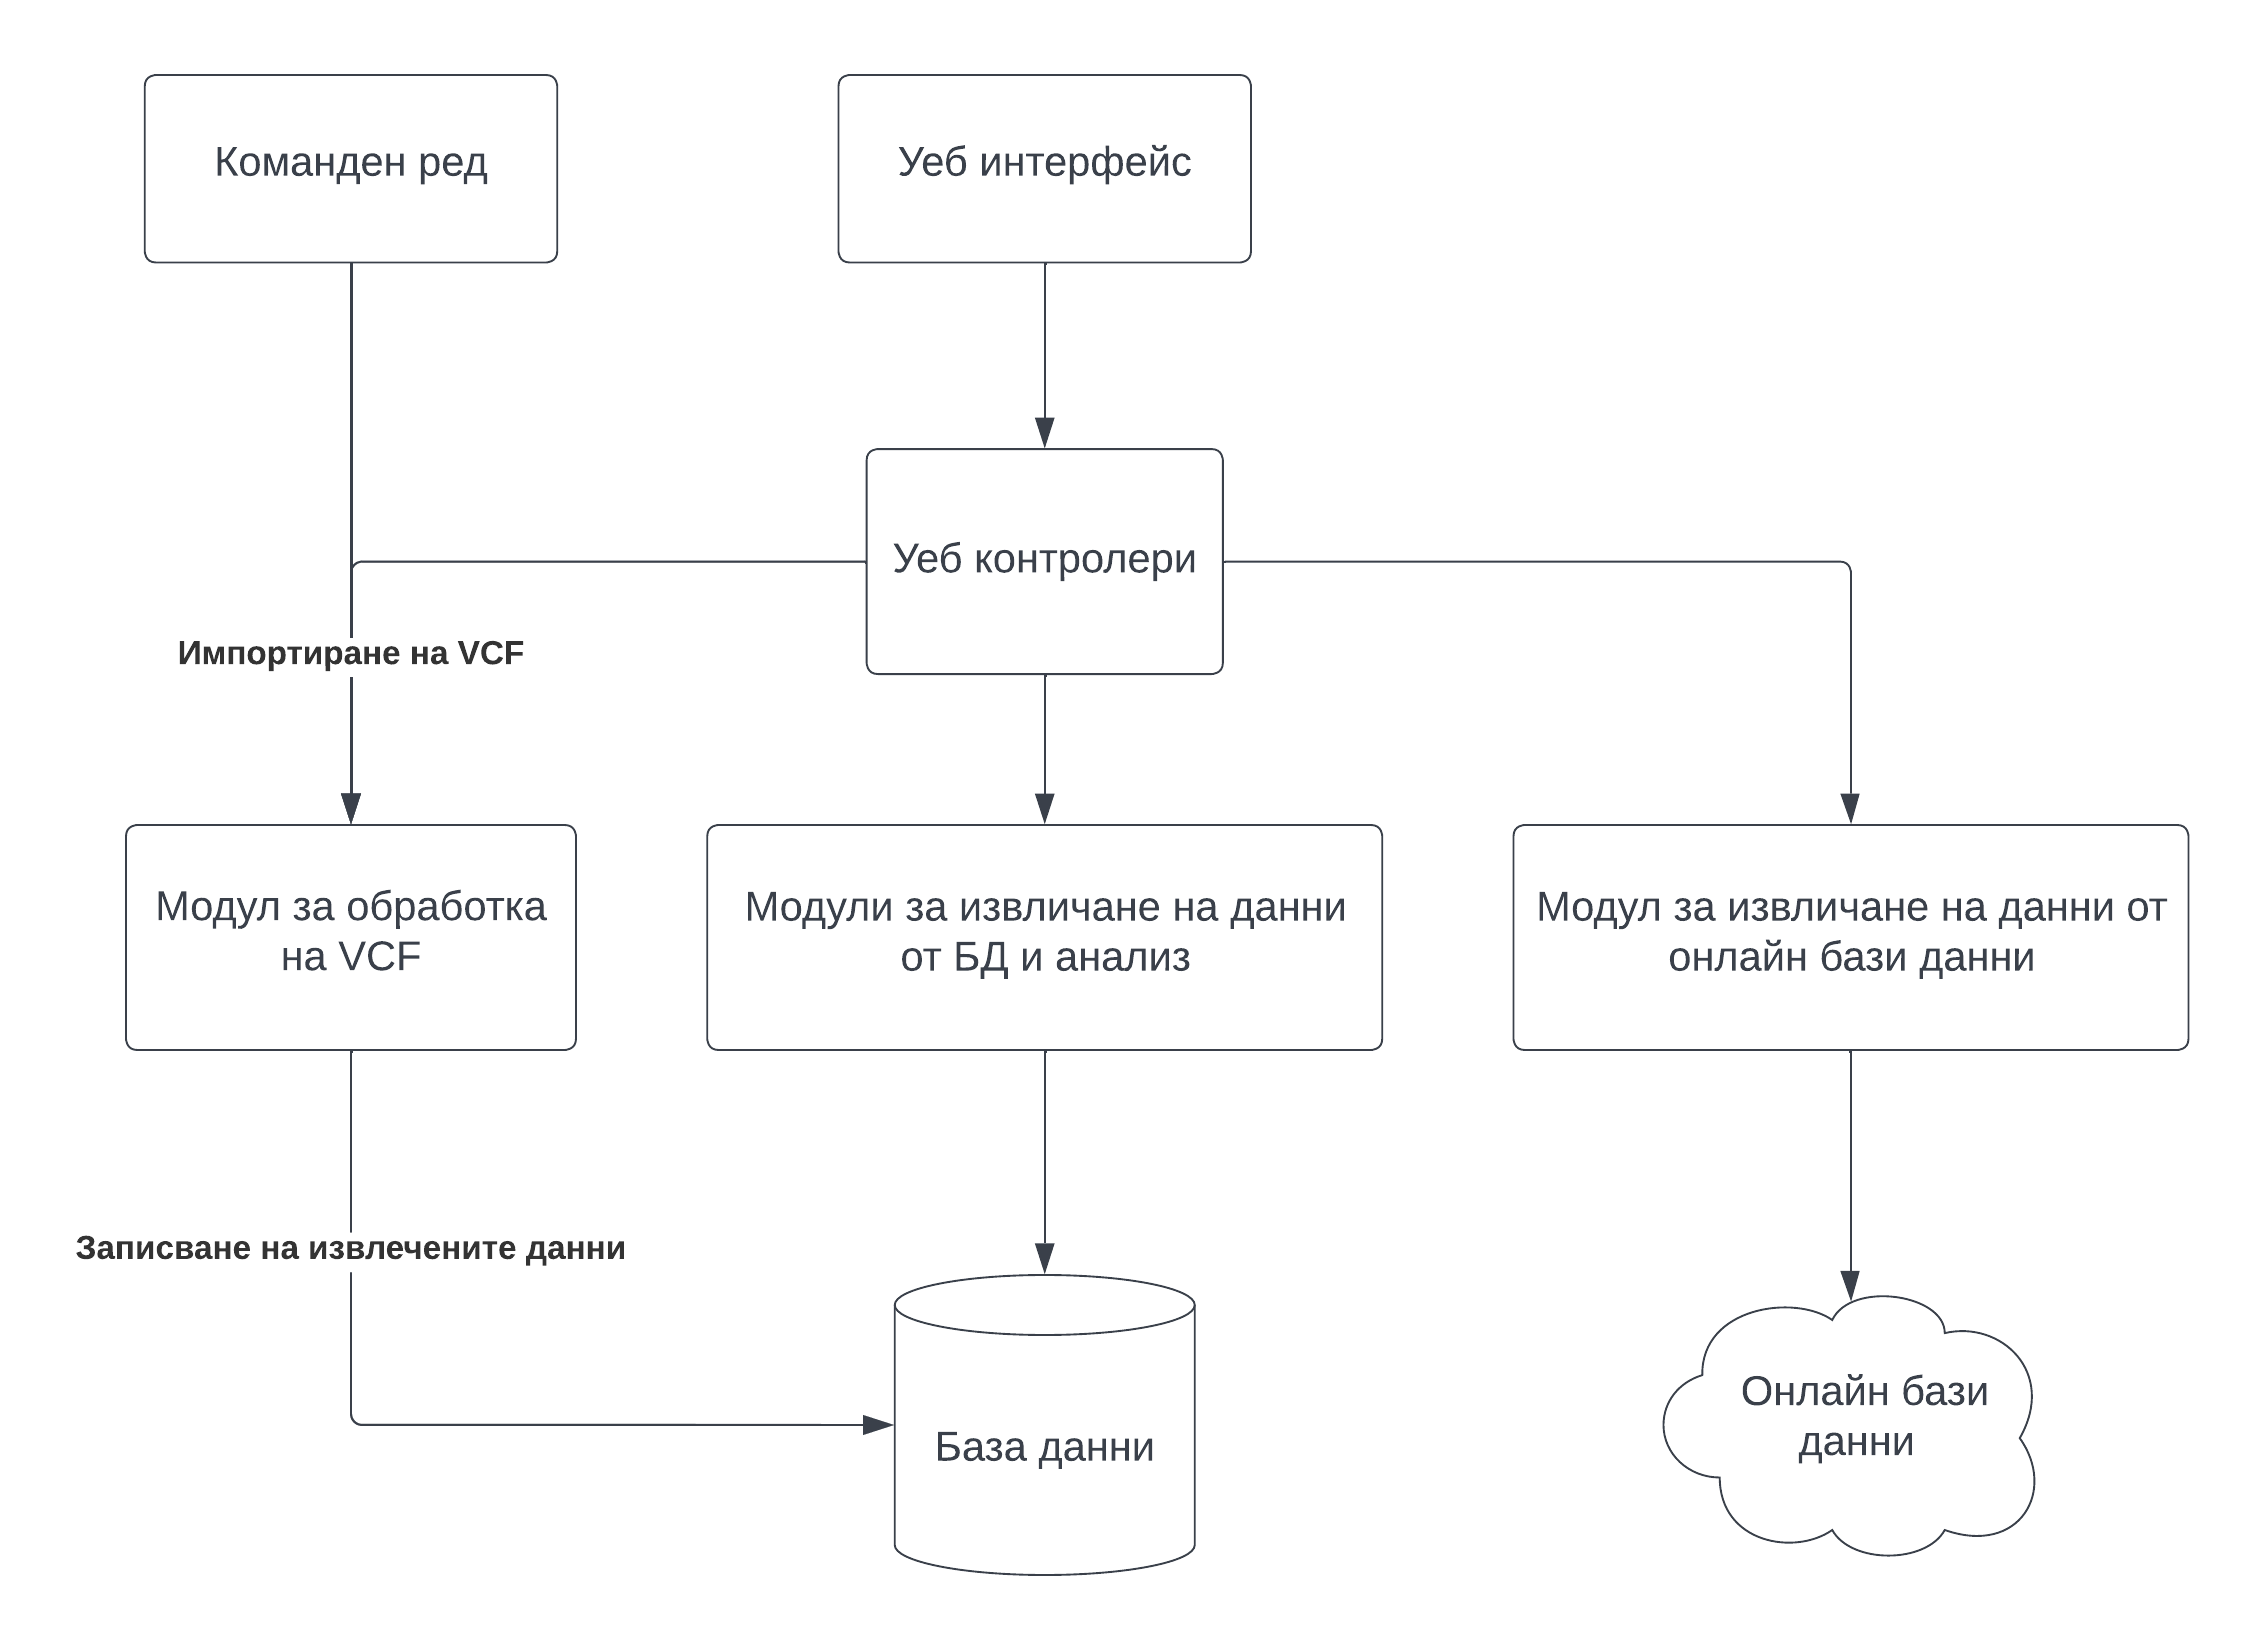
\includegraphics[width=17cm]{figures/software_architecture}
  \caption {Диаграма на софтуерната архитектура на разработеното решение}
  \label{fig:software_architecture}
\end{figure}

\section{База данни}
При изборът на тип на базата данни се спряхме на релационна база данни. Причините за това са няколко. Първата съществена причина е това, че структурата на данните е предварително ясна и промени по нея са малко вероятни. Това е така, тъй като структурата е базирана на информацията налична във VCF файловете и тази, предоставяна от софтуера за анотация (SnpEff). VCF форматът е дефиниран в общоприет стандарт \cite{danecek2011variant}, който не се променя често. Анотациите, предоставяни от SnpEff, също спазват определен стандарт \cite{cingolani2018variant}. Втората причина е, че релационните бази данни позволяват моделиране на базата спрямо концептуалния модел на данните, докато заявките, които ще се изпълняват, могат да имат по-малко значение \cite{chebotko2015}. Това свойство на релационните бази данни е подходящо за нашия случай, при който от самото начало е ясно с какви данни разполагаме, но не и как точно можем да ги анализираме. Релационната база данни ни позволява лесно да добавим нови заявки, без да са необходими промени по структурата на базата данни. Третата причина е, че не предвиждаме работа с толкова големи обеми от данни, че да изискват дистрибутиране на базата данни върху различни сървъри.

\paragraph{}
Измежду множеството релационни бази данни се избрахме DuckDB. Причините за това са свойството ѝ да се вгражда в друга програма, без да е необходим отделен сървър за управление на базата данни, което улеснява инсталацията, и поради приложимостта ѝ за изпълняване на аналитични заявки (виж секция \ref{sec:duckdb}).

\paragraph{}
Таблиците, използвани в програмното решение, могат да се разделят на две групи: такива, които са свързани с дефинирането на генни множества, и такива, които съхраняват информацията от анотирани VCF файлове с генетични варианти. За дефинирането на генни множества се използва таблица за множеството и втора таблица за членовете на множествата, като съществува 1-към-N релация между двете (фиг. \ref{fig:db_diagram}). Информацията за всеки анотиран VCF файл с генетични варианти може да се представи като йерархична структура: файлът включва множество гени, всеки от които е засегнат от множество варианти, а всеки варинт може да притежава много анотации (фиг. \ref{fig:annotated_vcf_hierarchy}). Съответно, тази йерархия е моделирана поседством четири таблици: файлове, гени, варианти и анотации. Всяка от тях съдържа външен ключ към предишната и по този начин образува N-към-1 релация с нея.

\begin{figure}[htp]
  \centering
  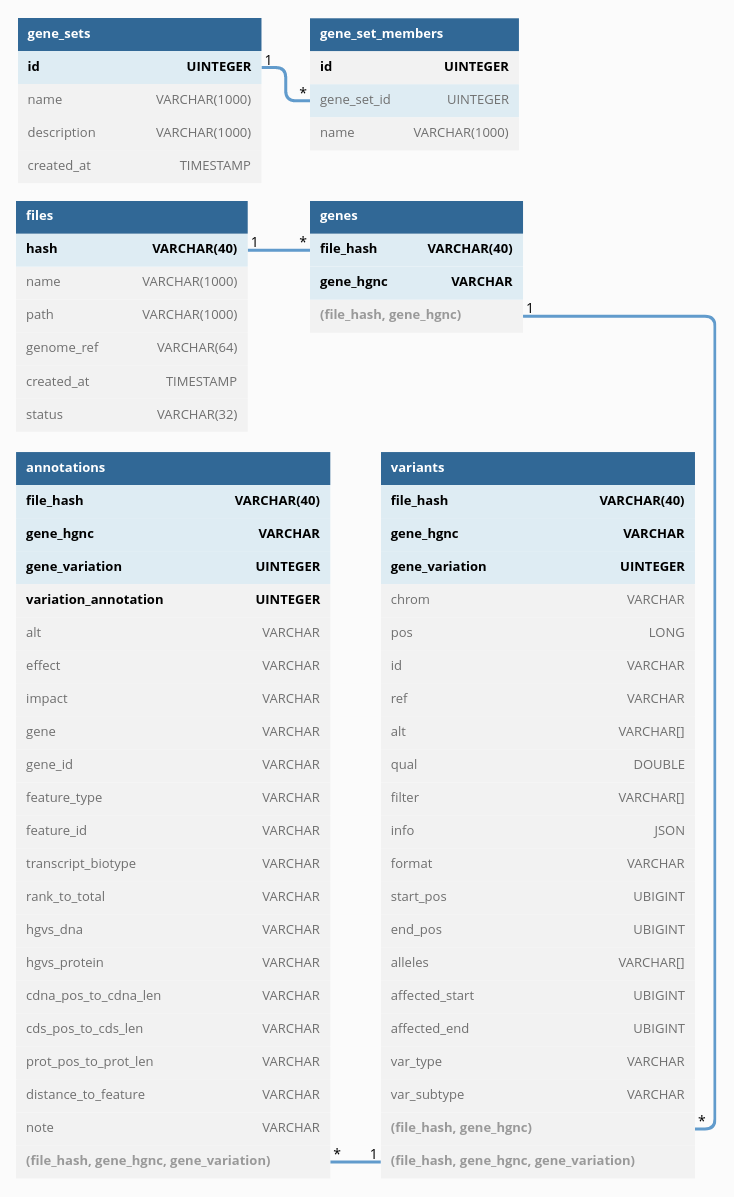
\includegraphics[width=14cm]{figures/db_diagram}
  \caption {Диаграма на структурата на базата данни}
  \label{fig:db_diagram}
\end{figure}

\begin{figure}[h]
  \centering
  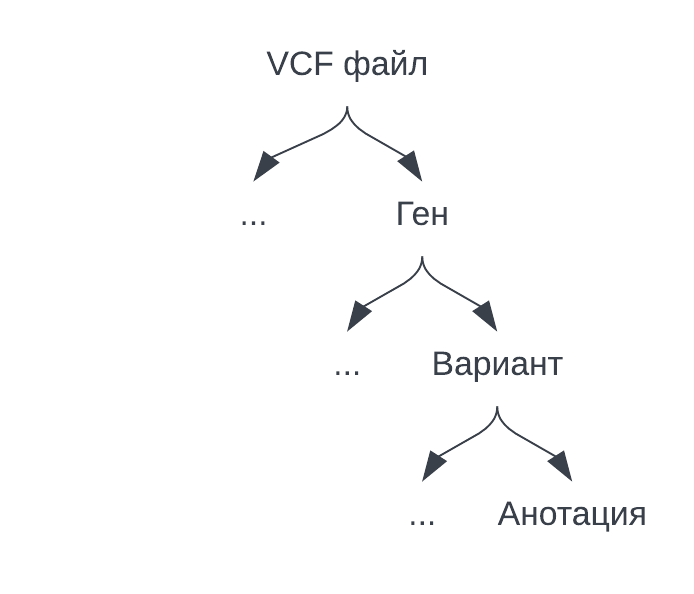
\includegraphics[width=6cm]{figures/annotated_vcf_hierarchy}
  \caption {Йерархично представяне на информацията от анотиран VCF файл}
  \label{fig:annotated_vcf_hierarchy}
\end{figure}


\section{Управление на генни множества}\label{sec:gene_sets}
\paragraph{}
Възможността за управление на генетични множества е проста функционалност, която позволява на потребителя да създава, редактира и изтрива колекции от гени, които представляват цел за някакви изследвания. Всяко генно множество има име, описание и списък от HGNC символи на гени. Дефинирането на генно множество става посредством качване на файл, съдържащ един HGNC символ на ред. В последствие, когато качва VCF файл с генетични множества за обработка, потребителят избира спрямо кое генетично множество да бъде обработен VCF файла. Единствено варианти свързани с гените от това множество ще бъдат запазени в базата данни. Тази, макар и проста функционалност, прави програмното решение по-генерализирано и позволява изследването на различни биологични процеси. Например, ако потребителят качи списък от гени, свързани с ракови заболявания, ще може да изследва полиморфизми за тяхната връзка с рака.

\section{Обработка на VCF при импортиране}
\paragraph{}
Началната точка при работа с разработения софтуер е качване на VCF файл, съдържащ генетични варианти. Това може да бъде направено както с уеб интерфейса, така и с интерфейсът, използваш командния ред (всъщност, импортирането и обработването на VCF е единствената операция, която командния ред може да извършва към момента). При качването на входен VCF файл за обработка, потребителят подава и генно множество, определящо кои гени да бъдат разгледани при обработката (виж секция \ref{sec:gene_sets}).

\paragraph{}
Първата стъпка, която се извършва при обработката на входния VCF е проверка, дали същият файл вече е бил изследван. За целта се калкулира неговата SHA256 хеш сума. Тази сума се използва като главен ключ на таблицата с файлове в базата данни. Ако сумата вече съществува в базата данни, значи файлът вече е бил импортиран и обработката приключва. Ако файлът не е срещан досега, обработката продължава. Прави се валидация, която проверява, че файлът не използва твърде стара версия на VCF стандарта (поддържат се версии не по-малки от 4.0), и се извлича информация за това спрямо кой референтен геном е създаден файлът (фиг. \ref{fig:vcf_processing_sequence}).

\paragraph{}
Следва същинската обработка на входния VCF файл. Първо, външните програми SnpEff и SnpSift, съответно за анотация и филтриране, биват стартирани като отделни процеси. Двата процеса биват свързани посредством pipe оператор, така че анотираните VCF редове, които SnpEff връща, да се подадат директно като входни данни за SnpSift. По този начин SnpEff добавя анотация към редовете на входния VCF, която включва и HGNC символа на гена, с който дадения вариант е свързан. SnpSift филтрира редовете, които му се подават, като оставя само тези, които се отнасят за гени, включени в генното множество, което потребителят е избрал. Резултатът се чете от основната програма, която разглежда всеки ред за да определи за кой ген се отнася и го записва в нов частичен VCF файл, който съдържа само вариантите за дадения ген. Резултатът от тези стъпки е колекция от VCF файлове, всеки от които е анотиран и съдържа само генетичните варианти за един единствен ген. Следващата стъпка е обхождането на всеки от тези файлове, изчитането на данните в Pandas DataFrame обект, който преминава поредица трансформации, и записването на крайната информация в базата данни. Също така, за всеки от тези VCF файлове се създава минимизирана версия, която изключва вариантите определени като незначителни от SnpEff (по-конкретно, за които полето impact има стойност „MODIFIER“). Тази минимизирана версия по-късно се използва за зареждане на генетичните варианти в геномния браузър, като по този начин се осъществява оптимизация на производителността и намаляване на шума за потребителя. Минимизираният и пълният VCF файлове за всеки ген също така се компресират и индексират посредством tabix функционалността (виж секция \ref{sec:samtools_tabix}), предоставяна от модула pysam (виж секция \ref{sec:pysam}). Компресията служи за оптимизация на изискванията към хардуерните ресурси, а създаването на индексни файлове е необходимо за да могат по-късно файловете да се зареждат и визуализират от геномния браузър.

\begin{figure}[htp]
  \centering
  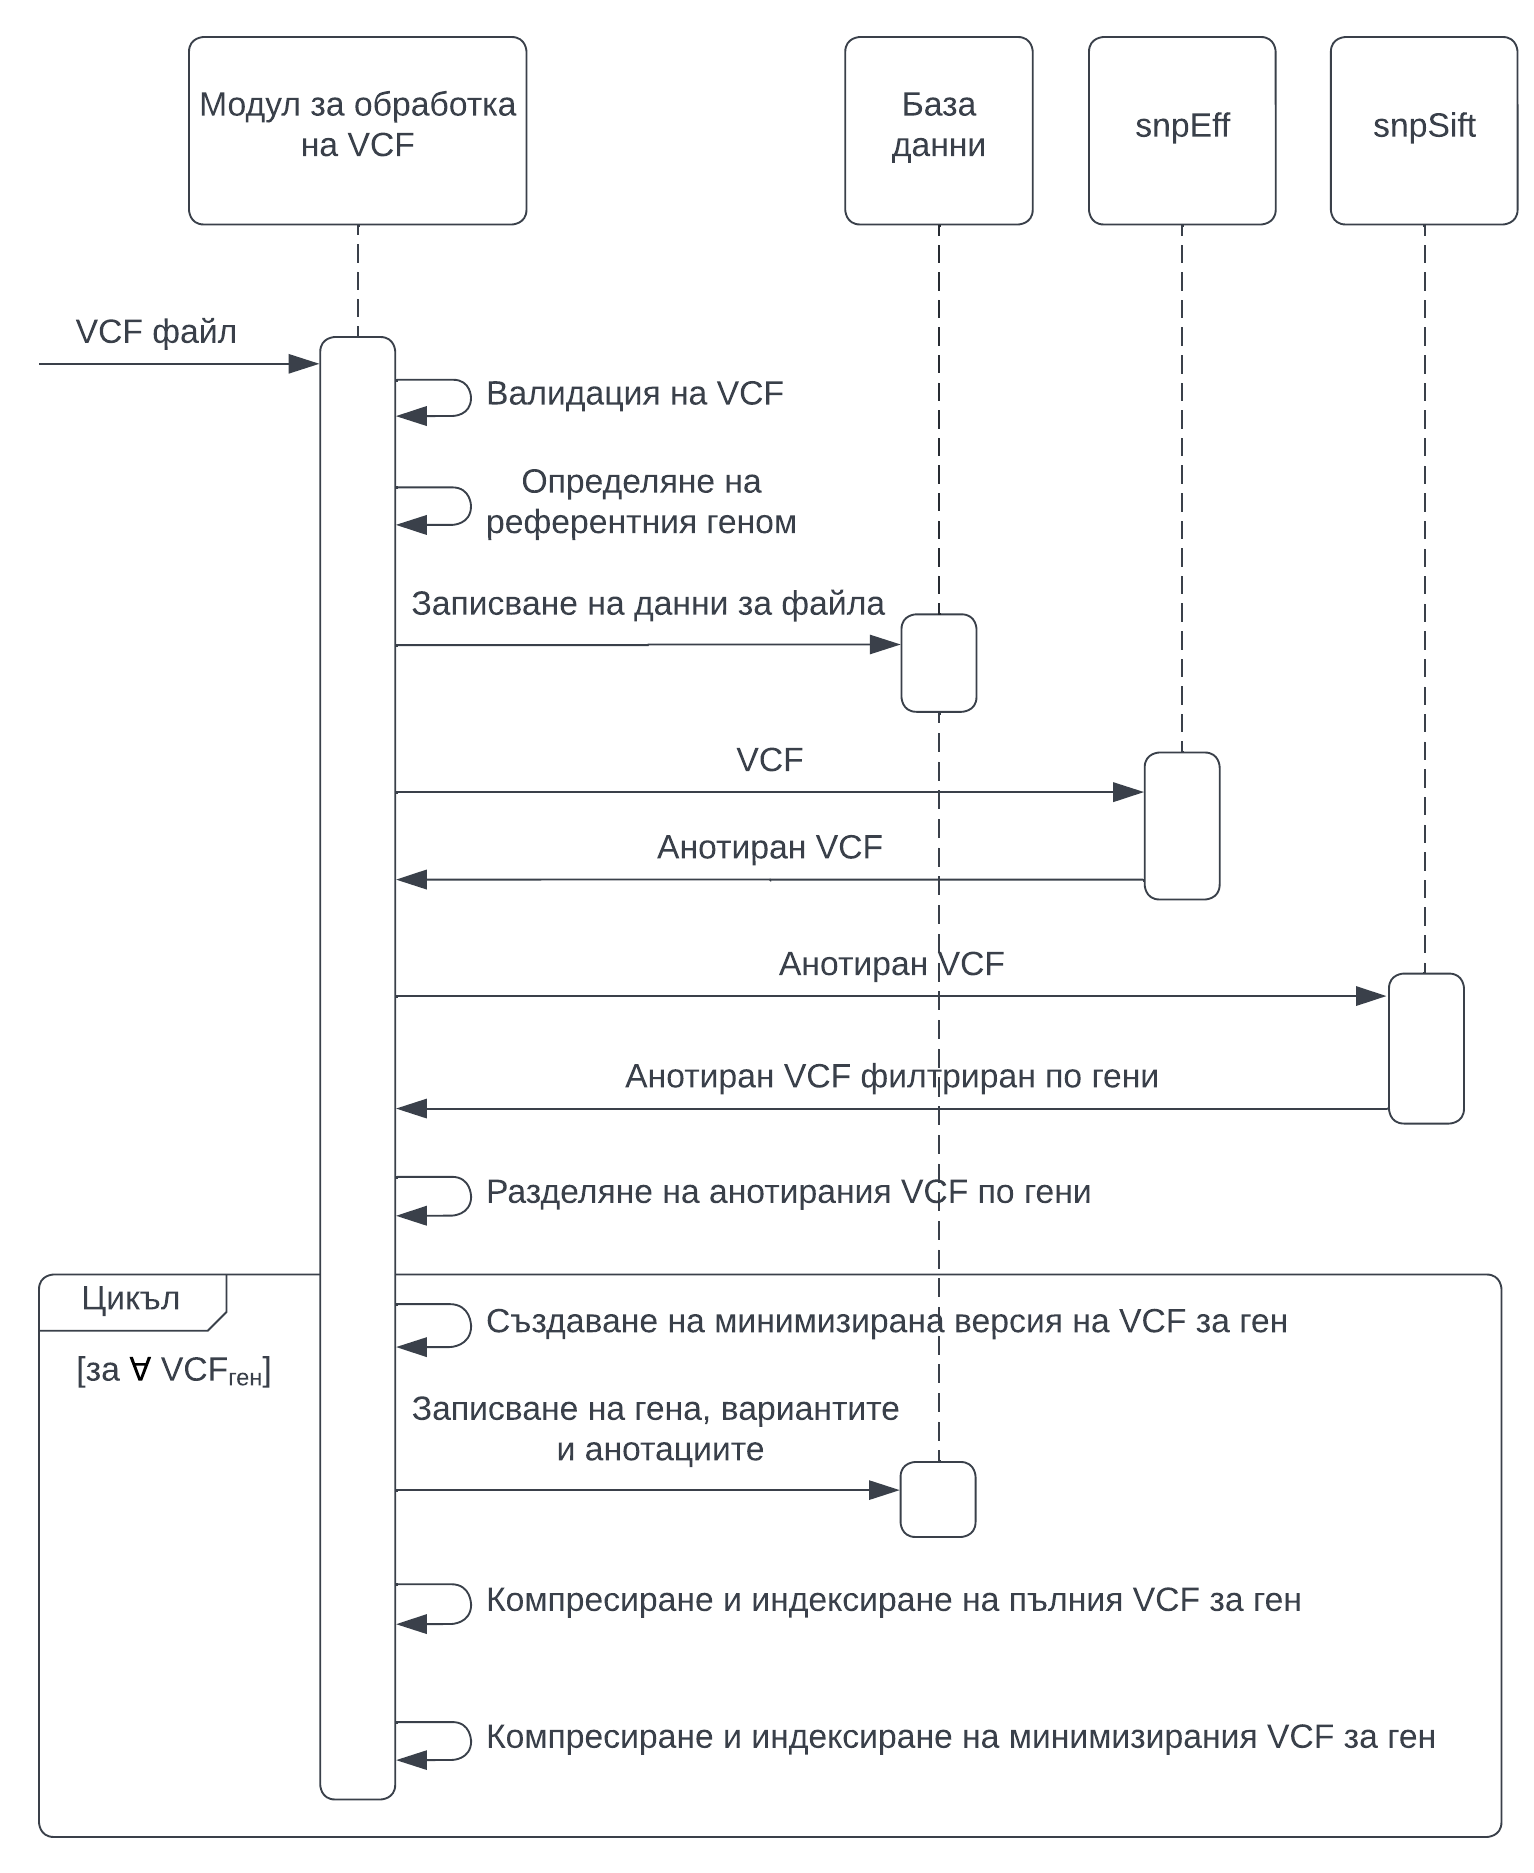
\includegraphics[width=16cm]{figures/vcf_processing_sequence}
  \caption {Диаграма показваща опростено описание на процеса по обработка на VCF файлове с генетични варианти.}
  \label{fig:vcf_processing_sequence}
\end{figure}

\section{Операции върху импортиран VCF}
\paragraph{}
След като един входен VCF, съдържащ генетични варианти, бъде импортиран и обработката му приключи, потребителят може да изследва резултатите. В тази секция са представени основните функции, които програмното решение предоставя.

\subsection{Списък на файлове}
Началната страница предоставя списък с наличните файлове, които вече са импортирани. Потребителят може да избере дали да изследва данните за някой от наличните файлове, да стартира обработката на нов файл или да изтрие информацията за съществуващ файл (фиг. \ref{fig:list_files}).

\subsection{Обзор на файл}
\paragraph{}
Страницата за обзор на файл дава най-обща информация за вече обработен файл. Това включва референтния геном, спрямо който файлът е създаден, генното множество, спрямо което е изследван, броя гени засегнати от полиморфизми и броят анотации. По-детайлна разбивка е дадена в табличен вид, която показва за всеки ген броя варианти и техните анотации спрямо оценената им тежест (фиг. \ref{fig:file_summary}).


\subsection{Обзор на ген}
\paragraph{}
Страницата за обзор на ген дава обща информация за гена и служи като отправна точка за изследването на различните варианти във файла, които го засягат. Страницата предоставя връзки към различни стандартни онлайн бази данни, където потребителят може да открие допълнителна информация за конкретния ген. Тези връзки включват базите данни Ensembl (виж секция \ref{sec:ensembl}), Entrez, HGNC (виж секция \ref{sec:hgnc}) и UniProt. Следва списък от богата анотация за протеина, кодиран от гена, включваща молекулярната функция, процесите и биологичните пътища, в които участва, каталитичната дейност и др (фиг. \ref{fig:gene_summary}). Налична е връзка към страницата, представяща всички варианти за гена.

\paragraph{}
Страницата включва и по-детайлна разбивка на анотираните варианти за гена, представени в табличен вид. Таблицата показва броят на анотациите за варианти, групирани по оценка на тежестта и генетичен ефект. Оценката на тежестта може да е четири варианта: модификатор, ниска, средна, висока. Възможните ефекти са разнообразни и включват например: синонимни мутации, придобиване на стоп кодон, мутации, изменящи смисъла или изместващи рамката, мутации в интрони и др (фиг. \ref{fig:gene_effects}). Всяка от стойностите в таблицата представлява връзка, при натискането на която, потребителят бива препратен към страницата за варианти, като се добавя филтър за конкретната стойност, така че потребителят да може да разгледа точно този вид варианти.

\subsection{Варианти на ген}
\paragraph{}
В страницата за варианти да ген потребителят има достъп до геномен браузър, чрез който може да изследва полиморфизмите засягащи гена. При отварянето на страницата, браузърът автоматично се фокусира върху геномния регион, съдържащ списъка от варианти във VCF файла. Геномният браузър представя няколко различни информационни ленти. Първата лента показва генните варианти. Тъй като VCF файлът може да е за един експеримент, или множество експерименти, тази лента показва също така и комбинациите от изразени варианти за всеки от експериментите във VCF файла. Втората лента показва гените, като са обособени техните екзони и интрони. Третата лента показва транскриптите, които се кодират от даден ген, заедно с техните Ensembl идентификатори (фиг. \ref{fig:genome_browser}).

\paragraph{}
В страницата също е налична странирана таблица с всички варианти за гена. Таблицата представя началната и крайната точка на полиморфизма, референтната и алтернативната нуклеотидна поредица, типа и подтипа на полиморфизма (точкова мутация, вмъкване, изтриване и тн.). Налични са и контроли, с които могат да бъдат прилагани сложни филтри върху данните от таблицата (фиг. \ref{fig:variants_list}).

\subsection{Засегнати транскрипти}\label{sec:affected_transcripts}
\paragraph{}
За всеки генетичен вариант можем да достъпим страница със засегнатите от него транскрипти. Страницата предоставя таблица с Ensembl идентификатора на транскрипта, неговия тип (например протеинокодиращ, псевдоген и тн), ефекта, който полиморфизма оказва върху този транскрипт, тежеста на промяната и HGVS номенклатура (виж секция \ref{sec:hgvs}) на промяната на протеина, ако има такава. Потребителят също така може да сравни и референтния и алтернативния протеин за този транскрипт (фиг. \ref{fig:protein_comparison}).

\subsection{Нагъване на протеини}
\paragraph{}
Беше разгледана и възможността за интегриране на софтуер за нагъване на протеини на база протеиновата секвенция, както и софтуер за визуализация на получените триизмерни структури. Както става ясно от секция \ref{sec:affected_transcripts}, системата ни има способността да изведе референтната и алтернативната протеинови секвенции. Тези секвенции могат да бъдат подадени като входни данни на програма за нагъване на протеини. За целта се спряхме на програмата AlphaFold, която към днешна дата предлага най-висока точност на резултатите (виж секция \ref{sec:alphafold}). Макар да успяхме да използваме AlphaFold2 за предсказване на третичната структура на протеини (фиг. \ref{fig:folded_protein}), в крайна сметка заключихме, че интегрирането ѝ в софтуерното решение не достатъчно практично на този етап. Причините за това са сравнително трудната инсталация, необходимостта от сваляне на огромни бази данни (дори опцията използваща редуцирана база данни изисква над 600GB бази данни) и голямата продължителност на процеса по нагъване на протеини. На компютърна конфигурация с процесор CPU Ryzen 7 5800X (AM4/4,7GHz/36MB), 32 GB RAM и HDD със скорост 175 MB/s, нагъването на неголям протеин с 600 аминокиселини отнема около 100 минути.

\begin{figure}[h]
  \centering
  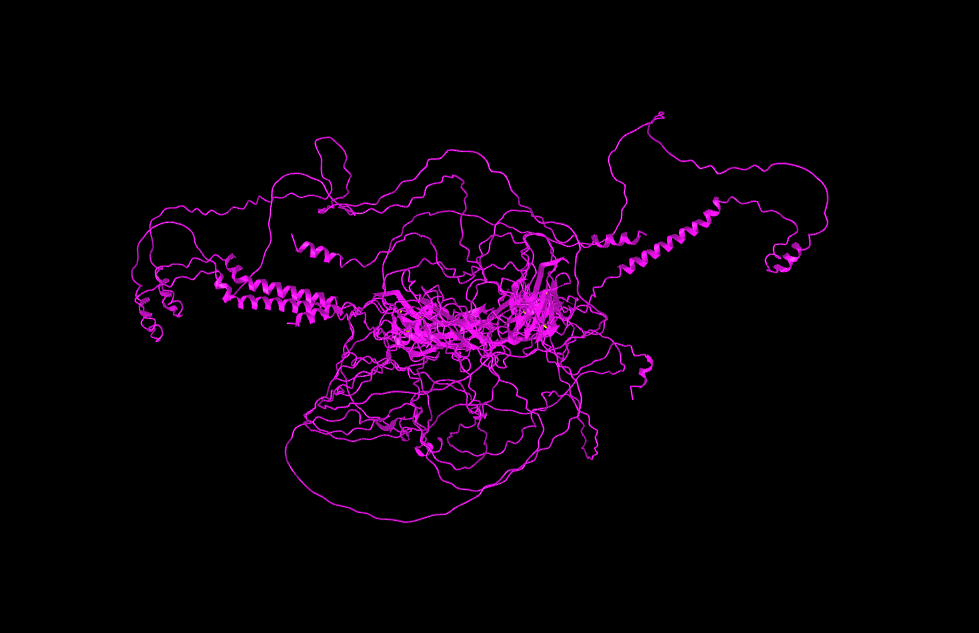
\includegraphics[width=16cm]{figures/folded_protein}
  \caption {Пример за предсказаната триизмерна структура на протеина GHR (P10912), получена чрез AlphaFold2.}
  \label{fig:folded_protein}
\end{figure}

\chapter{Заключение}
\paragraph{}
Дипломната работа устаноява наличието на богата екосистема от различни инструменти и биоинформатични програми, които покриват различните аспекти от обработката и анализа на генетични варианти. Макар да не предоставя нови възможности, които досега са липсвали изцяло, разработеният софтуер дава възможност за изключително лесно и бързо изследване на данните, без да изисква никакви специализирани познания по информатика и програмиране. В контраст, вече съществуващите решения най-често предлагат интерфейс, използващ командния ред на операционната система, а дори прост анализ изисква комбинирането на няколко различни програми. Алтернативите, предлагащи по-удобен графичен потребителски интерфейс, като Galaxy, също включват множество разнообразни и не съвсем интегрирани инструменти, което ги прави сравнително сложни за използване.

\paragraph{}
Разработената интегрирана система прави изследването на генетични варианти по-достъпно и удобно, но е лишена от гъвкавостта и голямото разнообразие от възможности, което съществуващите алтернативи предлагат. Това я прави подходящ избор за потребители, които нямат добри информатични познания, или за такива, които имат, но искат да направят първоначално обследване на данните, преди да изградят по-специализирана система за биоинформатична обработка.

\paragraph{}
Разработената система надскача поставените цели, като дава възможност за изследване на генетични варианти свързани с произволни биологични функции, а не само на такива свързани със процеса на стареене. Това е възможно благодарение на функционалността за управление на генетични множества, която позволява на потребителя да анализира генетичните варианти спрямо определен от него списък от гени.

\paragraph{}
Други от поставените цели не са постигнати и остават обект на бъдещи развития на софтуерното решение. Такива са разработването на потребителски интерфейс, използващ командния ред, чрез който системата да може да бъде програматично свързвана в по-мащабни биоинформатични системи. Също така, макар да бе разгледана възможността за интегрирането на програма за предсказване на триизмерната структура на протеини и на такава за визуализирането ѝ в софтуерното решение, това в крайна сметка се оказа непрактично и не бе осъществено.

\paragraph{}
Бъдещи разработки могат да допринесат към развитието на софтуерното решение в редица различни направления. Добаяването на възможност за изследване на епигенетични изменения е едно от тях. Смята се, че съществува значителна връзка между стареенето и процеса на ДНК метилирането, който е един от най-важните епигенетични процеси. VCF файловете, които са основните входни данни за разработената система, се използват и за отчитането на нивата на ДНК метилиране при бисулфатно секвениране на целия геном \cite{barturen2013}\cite{merkel2018}. Разширяването на възможностите на системата, така че да може да обработва и такива VCF файлове, би ѝ дало значително предимство.

\paragraph{}
Друго възможно бъдещо развитие на изградената системата е добавянето на функционалности за популационна генетика. VCF файловете могат да съдържат информация за един или много индивиди. Би било полезно ако системата може да идентифицира файловете съдържащи данни за генетични варианти сред група индивиди и предоставя колекция от функционалности даващи различни статистики и анализи от областта на популационната генетика.

\chapter{Изводи}
\begin{enumerate}
	\item Проектирана и изградена е софтуерна система, която интегрира множество съществуващи решения, за да предостави достъпен и лесен за използване инструмент за анализ на генетични варианти.
	\item Изградената система предлага сравнително базови функционалности, които я правят полезен иснтрумент за генетични анализи от учени без дълбоки познания по информатика, както и експерти с добра биоинформатична подготовка.
	\item Системата служи като база за бъдещи разработки, които да предоставят възможности за улесняване на изследванията в области като епигенетика, популационна генетика и други.
\end{enumerate}


\cleardoublepage
\phantomsection
\addcontentsline{toc}{chapter}{Библиография}
\bibliographystyle{unsrt}
\bibliography{refs}


\cleardoublepage
\chapter*{Приложение}
\phantomsection
\addcontentsline{toc}{chapter}{Приложение}

\begin{figure}[h]
  \centering
  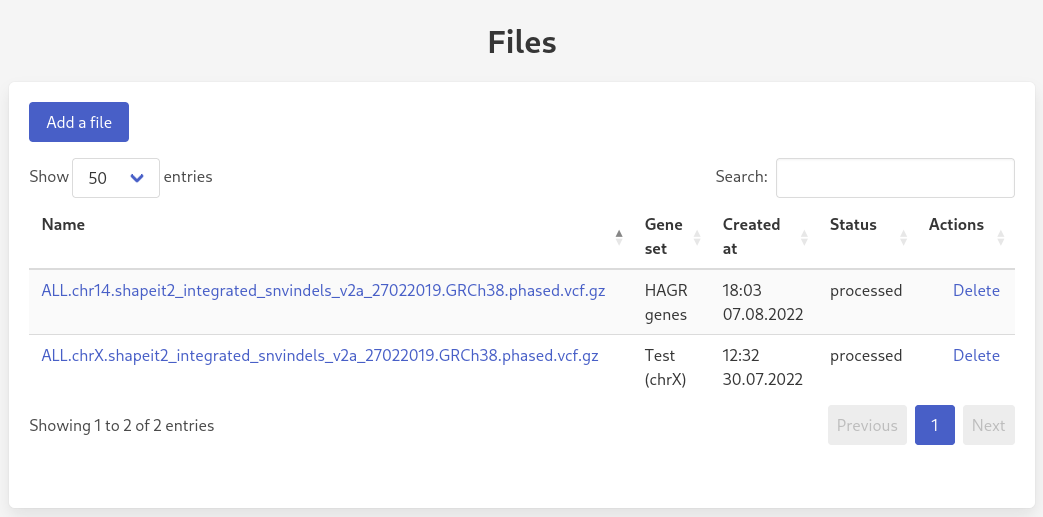
\includegraphics[width=16cm]{figures/list_files}
  \caption {Списък от файлове.}
  \label{fig:list_files}
\end{figure}


\begin{figure}[ht]
  \centering
  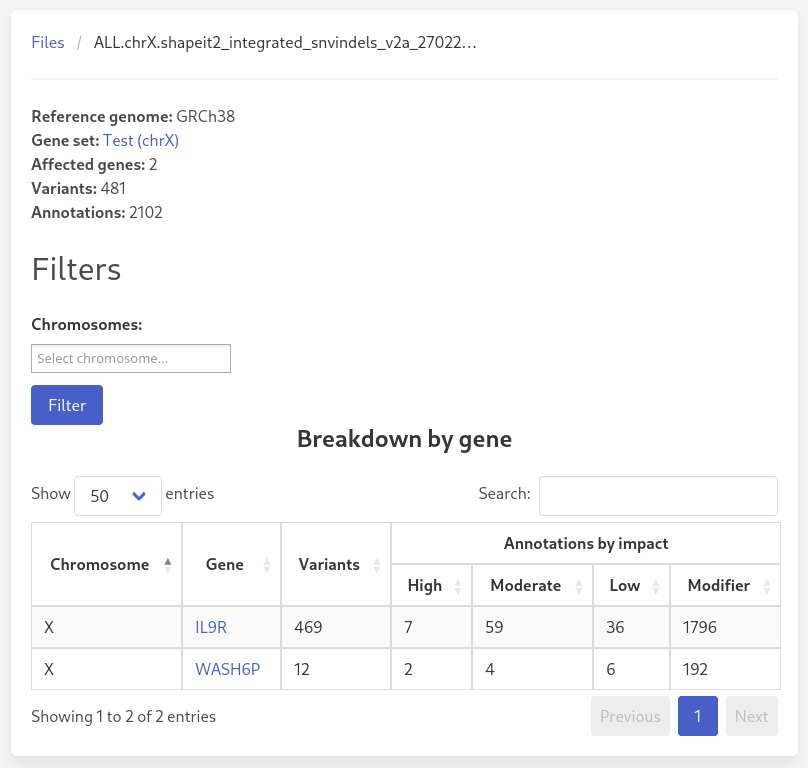
\includegraphics[width=16cm]{figures/file_summary}
  \caption {Обзор на файл.}
  \label{fig:file_summary}
\end{figure}

\begin{figure}[ht]
  \centering
  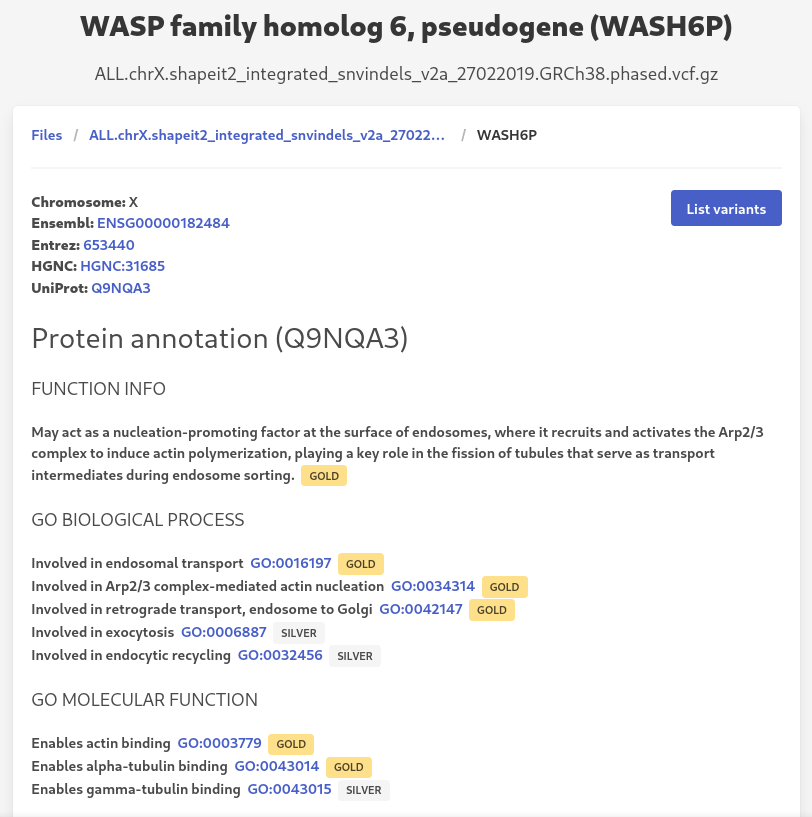
\includegraphics[width=16cm]{figures/gene_summary}
  \caption {Обща информация за гена.}
  \label{fig:gene_summary}
\end{figure}

\begin{figure}[ht]
  \centering
  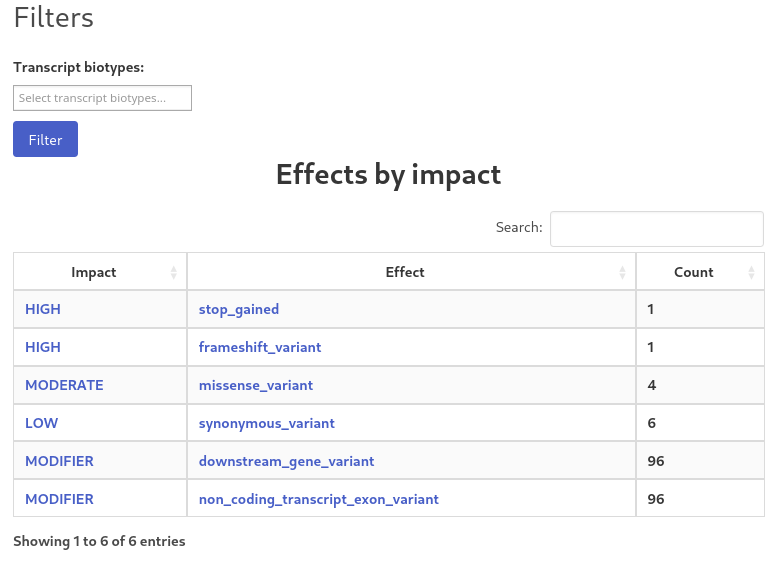
\includegraphics[width=16cm]{figures/gene_summary_effects}
  \caption {Разбивка на анотираните варианти и техните предсказани ефекти.}
  \label{fig:gene_effects}
\end{figure}

\begin{figure}[ht]
  \centering
  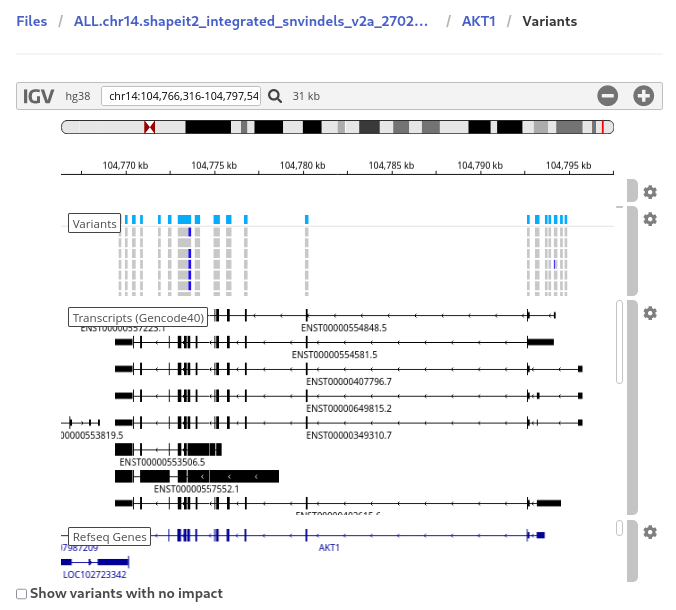
\includegraphics[width=16cm]{figures/genome_browser}
  \caption {Геномен браузър за изследване на генетичните варианти.}
  \label{fig:genome_browser}
\end{figure}

\begin{figure}[ht]
  \centering
  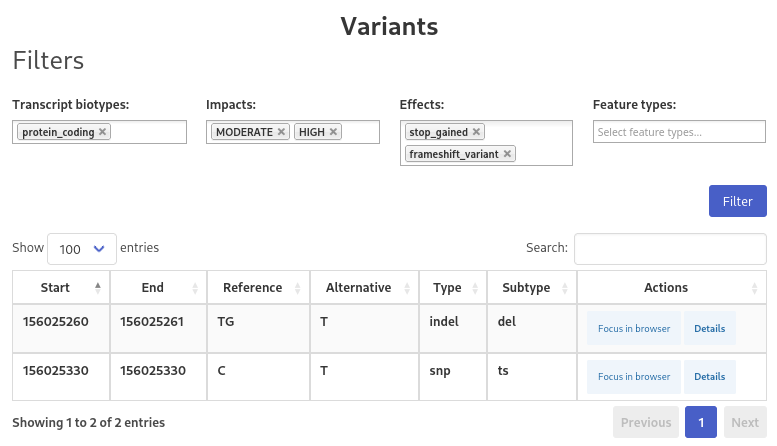
\includegraphics[width=16cm]{figures/variants_list}
  \caption {Таблица с геномни варианти и филтри.}
  \label{fig:variants_list}
\end{figure}

\begin{figure}[ht]
  \centering
  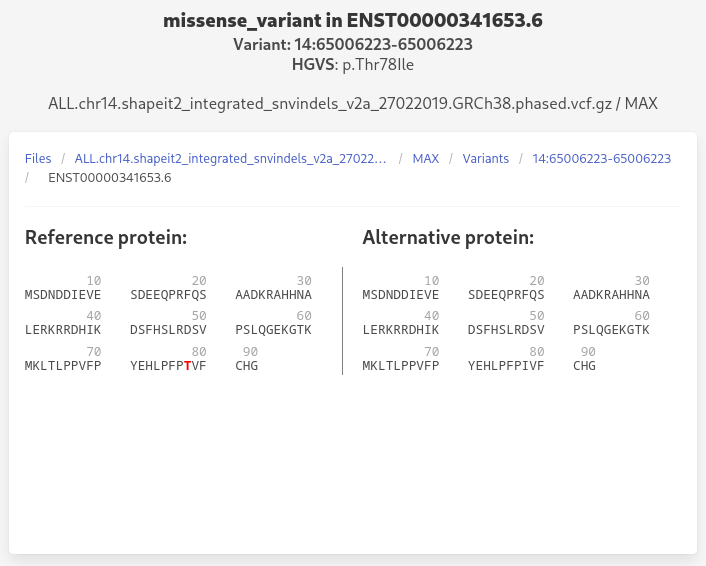
\includegraphics[width=16cm]{figures/protein_comparison}
  \caption {Сравнение на референтен и алтернативен протеин. Мястото на полиморфизма е оцветено в червено.}
  \label{fig:protein_comparison}
\end{figure}

\end{document}